\documentclass[10pt, spanish]{report}
\usepackage[none]{hyphenat}
\usepackage[utf8]{inputenc}
\usepackage[T1]{fontenc}
\usepackage[spanish]{babel}

\usepackage{geometry}
\def \margin {20mm}
\geometry{
    a4paper,
    left=\margin,
    right=\margin,
    top=\margin,
    bottom=\margin
}

\usepackage{lmodern}
\usepackage{xfrac}

\usepackage{enumitem}
\renewcommand{\labelenumi}{(\theenumi)}
\renewcommand{\labelenumii}{(\theenumii)}

\usepackage{multicol}

% \setitemize{label=---,leftmargin=0.6cm}

\usepackage{amssymb}
\usepackage{mathtools}

\usepackage{marginnote}

%For left superscripts
\usepackage{leftidx}

\makeatletter
\renewcommand{\@makechapterhead}[1]{%
\vspace*{50 pt}%
{\setlength{\parindent}{0pt} \raggedright \normalfont
\bfseries\huge\thechapter.\ #1
\par\nobreak\vspace{1em}}}
\makeatother

% Theorems
\usepackage{amsthm}
\usepackage{thmtools}
\newtheorem*{lema}{Lema}
\newtheorem*{prop}{Proposición}
\newtheorem*{tma}{Teorema}
\newtheorem*{cor}{Corolario}
\theoremstyle{definition}
\newtheorem*{defin}{Definición}
\newtheorem*{notacion}{Notación}
% \newtheoremstyle{custom}{\topsep}{\topsep}{}{}{}{.}{ }{}
% \theoremstyle{custom}
\newtheorem*{ej}{Ejemplo}
\newtheorem*{ejer}{Ejercicio}
\newenvironment{sol}{\textit{Solución.}}{\hfill$\square$}
% \theoremstyle{remark}
\newtheorem*{obs}{Observación}
\newtheorem*{nota}{Nota}

% No indentation: \setlength\parindent{0pt}
\usepackage{parskip}

\let\emptyset\varnothing

% Custom math commands
\newcommand{\N}{\mathbb{N}}
\newcommand{\Z}{\mathbb{Z}}
\newcommand{\Q}{\mathbb{Q}}
\newcommand{\R}{\mathbb{R}}
\newcommand{\C}{\mathbb{C}}
\newcommand{\F}{\mathbb{F}}
\newcommand{\K}{\mathbb{K}}
\let\L\undefined
\newcommand{\L}{\mathbb{L}}

\newcommand{\id}{\text{id}}
\newcommand{\im}[1]{\operatorname{im}\left(#1\right)}
\newcommand{\car}[1]{\text{car}(#1)}
\newcommand{\ord}[1]{\text{ord}(#1)}
\newcommand{\mcd}[1]{\text{mcd}(#1)}

\renewcommand{\geq}{\geqslant}
\renewcommand{\leq}{\leqslant}

\DeclareMathSymbol{*}{\mathbin}{symbols}{"01}

% Diagrams
\usepackage{tikz}
\usetikzlibrary{cd}

\newcommand{\fecha}[1]{\marginpar{\underline{#1}}}
% \newcommand{\fecha}[1]{{\hfill\large{#1/2021}}\\[-0.8em]\noindent\rule{17cm}{0.1mm}}
\newcommand{\completar}{\fbox{\textbf{¡Completar!}}}
\newcommand{\revisar}{\fbox{¡Revisar!}}

\title{Ecuaciones algebraicas}
\author{Apuntes de Adrián Lattes}
\date{2021}

\begin{document}
\maketitle

\chapter{Extensiones de cuerpos}
\fecha{15/02}
\section{Raíces de polinomios y extensiones de cuerpos}

\begin{defin}
    Decimos que un anillo unitario y conmutativo $(\F,+,*)$ es un
    \textit{cuerpo} si para todo $a\in \F\setminus\{0\}$ existe $a^{-1}\in
    \F\setminus\{0\}$ tal que $a*a^{-1}=1$ y $1\neq 0$.
\end{defin}

\begin{obs}
    Con la definición anterior, el anillo $\{0\}$ no es un cuerpo.
\end{obs}

\begin{prop}
    Si $\F$ es un cuerpo sus únicos ideales son $\left\{ 0 \right\}$ y $\F$.
\end{prop}
\begin{proof}
    Sea $I\subseteq \F$ un ideal distinto de $\left\{ 0 \right\}$ y $a\in
    I\setminus\{0\}$. Entonces todo $b\in\F$ se puede escribir como
    $b=(ba^{-1})a\in I$, de donde $\F\subseteq I$ y por tanto $I=\F$.
\end{proof}

\begin{defin}
    Un homomorfismo de anillos unitarios $f:A\to A'$ es una aplicación tal que
    para todos $a,b\in A$:
    \begin{enumerate}
        \item $f(a+a')=f(a)+f(a')$
        \item $f(a*a')=f(a)*f(a')$
        \item $f(1_A)=f(1_{A'})$
    \end{enumerate}
\end{defin}

\begin{lema}
    Si $\F$ y $\F'$ son dos cuerpos y $f: \F\to\F'$ es un homomorfismo de
    anillos (unitarios), entonces $f$ es inyectivo.
\end{lema}
\begin{proof}
    Sabemos por definición que $f(1)=1$, por lo que $1_\F\neq \ker{f}$ y
    $\ker{f}\neq \F$. Como además $\ker{f}$ es un ideal de $\F$ se tiene que
    $\ker{f}=\{0\}$ lo que equivale a que $f$ sea inyectivo.
\end{proof}

\begin{defin}
    Sean $\K$ y $\L$ cuerpos y $f:\K\to\L$ un homomorfismo de anillos. Decimos
    que $f$ define una \textit{extensión de $\K$ en $\L$}.
    Por el lema tenemos que $\K\cong f(\K)\subseteq \L$, por lo que
    identificaremos $\K$ con $f(\K)$ y escribiremos \[\K\subseteq \L.\]
\end{defin}

\begin{ej}
    $\Q\subseteq\R$, $\R\subseteq\C$.
\end{ej}

\fecha{16/02}

\begin{ej}
    Sea $\F$ un cuerpo, consideramos el anillo de polinomios $\F[x]$ y
    $\K$ el cuerpo de fracciones de $\F[x]$,
    \[\K=\left\{ \frac{p}{q}\mid p,q\in \F[x], q\neq 0 \right\}\]
    donde $\frac{p}{q} = \frac{p'}{q'}$ si $pq'=p'q$.
    En $\K$ definimos la suma y producto como
    \begin{align*}
        \frac{p}{q}+\frac{p'}{q'}&=\frac{pq'+p'q}{pq}\\
        \frac{p}{q}*\frac{p'}{q'}&=\frac{pp'}{qq'}
    \end{align*}
\end{ej}

\begin{obs}
    $\frac{p}{q}$ es la clase de equivalencia de $(p,q)$ via la relación
    $(p,q)\sim(p',q')$ donde $(p,q),(p',q')\in K[x]\times(K[x]\setminus\{0\})$
\end{obs}

\begin{notacion}
    Sea $\K$ un cuerpo denotamos el cuerpo de fracciones de $\K[x]$ como
    $\K(x)$.
\end{notacion}

\begin{ej}
    Si $\F=\Q$, $\frac{2+x+x^3}{1+x^2}\in \Q(x)$
\end{ej}

\begin{ejer}
    Sean $\K$ y $\F$ dos cuerpos. La aplicación $j:\F\to\K$ tal que $j(a)=
    \frac{a}{1}$ es un homomorfismo que define la extensión $\F\subseteq \K$.
\end{ejer}


\section{Construcción de $\C$ a partir de $\R$}

Sea $\C =\left\{ a+bi\mid a,b\in\R, i^2 = -1 \right\}$ veamos que $\C\cong
\frac{\R[x]}{I}$ donde $I=\langle x^2 +1\rangle=\left\{(x^2+1)g\mid g\in\R[x]
\right\}$. La relación de congruencia está definida para $p,q\in\R[x]$ como
\[p\sim_I q \Leftrightarrow p-q\in I\Leftrightarrow x^2+1\mid(p-q).\]

Dado $p\in\R[x]$ se puede escribir como $p=h(x)*(x^2+1)+bx+a$, de donde
$p\sim_I bx+a=r(x)$ y su clase de equivalencia es $p+I=\left\{ p\mid p-q\in
I\right\}=(a+bx)I$. Con esto vemos que el conjunto cociente
\[\frac{\R[x]}{I}=\left\{ p+I\mid p\in\R[x] \right\} \]
es un anillo con las operaciones
\begin{align*}
    (p+I)+(p'+I)&=(p+p')+I\\
    (p+I)*(p'+I)&=(p*p')+I
\end{align*}

\begin{obs}
    La aplicación $j:\R\to\frac{\R[x]}{I}$ tal que $a\mapsto a+I$ es un
    homomorfismo inyectivo de anillos.
\end{obs}

En lo siguiente denotamos la clase $a+I$ por $a$, para todo $a\in\R$ y
escribimos $\alpha = x+I$. Con esto la clase de un elemento $a+bx$ es
\[a+bx+I=a+I+(b+I)*(\alpha+I)=a+b\alpha\]
y las operaciones
\begin{align*}
    (a+b\alpha)+(a'+b'\alpha)&=a+a'+(b+b')\alpha\\
    (a+b\alpha)*(a'+b'\alpha)&=aa'+(ab'+a'b)\alpha+bb'\alpha^2
\end{align*}
Ahora $\alpha^2=(x+I)^2=x^2+I$ y $x^2=1(x^2+1)=-1$ por lo que $\alpha^2=x^2+I
=-1+I=-1$

Con esto tenemos que la aplicación $\frac{\R[x]}{I}\to \C$ tal que
$a+b\alpha\mapsto a+bi$ es un isomorfismo.

\section{El anillo cociente $\K[x]/\left<f\right>$}

Sea ahora $\K$ un cuerpo, $f\in\K[x]$ de grado $n\geq 1$ e $I=\langle f\rangle=
\left\{ g*f\mid g\in\K[x] \right\}$, consideramos la congruencia módulo $I$:
\[p\sim_I q\Leftrightarrow p-q\in I \Leftrightarrow f\mid(p-q)\]
donde $p,q\in\K[x]$. La clase de equivalencia de $p\in\K[x]$ es $p+I\coloneqq
\left\{q\in\K[x]\mid p\sim_Iq\right\}=\left\{p+g\mid g\in I\right\}$.

Se tiene entonces que \[\frac{\K[x]}{I}=\left\{ p+I\mid p\in\K[x] \right\}\] es
un anillo unitario y conmutativo con las operaciones definidas entre los
representantes. Así \[\frac{\K[x]}{I}=\left\{ a_0+a_1x+\ldots+a_{n-1}x^{n-1}+
I\mid a_0,\ldots,a_{n-1}\in\K \right\}\] donde las $a_i$ son las clases de los
restos de dividir por $f$ y $n=\deg{f}$.

Si denotamos $a+I$ por $a$ para todo $a\in\K$ y $x+I$ por $\alpha$ podemos
escribir \[\frac{\K[x]}{I}=\left\{ a_0+a_1\alpha+\ldots+a_{n-1}\alpha^{n-1}\mid
a_0,\ldots,a_{n-1} \in\K \right\}.\]

Además $f(\alpha)=0$ en $\frac{\K[x]}{I}$ ya que, si $f=c_0+c_1x+\ldots+c_nx^n$:
\begin{align*}
    f(\alpha)&=c_0+c_1\alpha+\ldots+c_n\alpha^n=c_0+I+(c_1+I)(x+I)+\ldots
    +(c_n+I)(x+I)^n\\
             &=(c_0+c_1x+\ldots+c_n+x^n)+I=f+I=0+I.
\end{align*}

\fecha{17/02}
\begin{defin}
    Un anillo $A$ es \textit{íntegro} si para todos $a,b\in A$ con $a\neq 0, b
    \neq 0$ entonces $ab\neq 0$.
\end{defin}

\newpage
\begin{prop}
    Sea $\K$ un cuerpo y $f\in \K$ de grado $n\geq1$. Son equivalentes
    \begin{enumerate}
        \item $\frac{\K[t]}{\left< f \right>}$ es un anillo íntegro.
        \item $\frac{\K[t]}{\left< f\right>}$ es un cuerpo.
        \item $f$ es irreducible.
    \end{enumerate}
\end{prop}

\begin{proof}\hspace{1em}
    \begin{itemize}[itemindent=36pt]
        \item[(2)$\implies$(1)] Todo cuerpo es anillo íntegro.
        \item[(1)$\implies$(3)] Si $f=g*h$ con $\deg{f}>\deg{g},\deg{f}\geq
            \deg{h}$ y sea $\alpha = x+\left< f \right> $ se tiene $f(\alpha)=0
            =g(\alpha)h(\alpha)$. Ahora $g+\left< f \right> = g(\alpha) \neq 0$
            ya que $f$ divide a $g$ y análogamente $h+\left< f \right> =
            h(\alpha)\neq 0$.
            Por tanto $A=\frac{\K[t]}{\left< f \right> }$ no es íntegro.
        \item[(3)$\implies$(2)] Sea $g\in \K[t]$  tal que $g+\left< f \right>
            =g(\alpha)\neq 0$. Vemos que $\exists(g(\alpha))^{-1}$ en
            $A=\frac{\K[t]}{\left< f \right> }$. Como $f$ es irreducible y
            $\neg f|g \implies \gcd(f,g)=1$. En $\K[t]$ tenemos la identindad de
            Bézout (gracias a que $\K$ es cuerpo), por lo que existen $p,q\in
            \K[t]$ tales que $pf+qg=1$.
            Ahora, como $f(\alpha)=0$, $q(\alpha)=q+\left< f \right>$  es el
            inverso de $g(\alpha)=g+\left< f \right>$ ya que $1=q(\alpha)
            g(\alpha)$.
    \end{itemize}
    \vspace{-1em}
\end{proof}

\begin{cor}
    Sean $\K$ un cuerpo y $f\in\K[t]$ irreducible, existe una extensión
    $\K\subseteq\L$ y $\alpha\in\L$ tales que $f(\alpha)=0$.
\end{cor}

\begin{proof}
    Tomamos el cuerpo $\frac{\K[t]}{\left< f \right> }$ y el polinomio
    $\alpha=t+\left< f \right>$  y aplicamos la proposición anterior.
\end{proof}

\begin{ej}
    Sea $f=t^2-2\in \Q[t]$. Si $\alpha=\sqrt{2}$, $f$  tiene una raíz en $\R$ y
    $f=(t-\sqrt{2})(t+\sqrt{2})$ en $\R[t]$.
\end{ej}

\begin{defin}
    Sea $\K$ un cuerpo y $f\in\K[t]$, se dice que $f$ se \textit{escinde} sobre
    $\K$ (o se \textit{descompone totalmente} sobre $\K$) si existen $\alpha_1,
    \ldots,\alpha_n\in\K$ y $a\in\K$ tales que
    \[f=a(t-\alpha_1)*\ldots*(t-\alpha_n).\]
\end{defin}

\begin{obs}
    La condición de la definición es equivalente a que $f$ tenga todas sus
    raíces en $\K$. Es decir, todos los factores irreducibles de $f$ en $\K[t]$
    tienen grado $1$.
\end{obs}

\begin{tma}
    Sea $\K$ un cuerpo y $f\in\K[t]$ de grado $n\geq1$. Entonces existe una
    extensión $\K\subseteq L$ tal que $f$ se escinde sobre $L$.
\end{tma}

\begin{proof}
    Por inducción sobre $n=\deg{f}$:
    \begin{itemize}[itemindent=30pt]
        \item[Si $n=1$] $f=a+bt$ con $b\neq 0$ y $f=b(\frac{a}{b}+t)$ y
            $-\frac{a}{b}$ es raíz de $f$.
        \item[Si $n>1$] Supongamos que el resultado es cierto para polinomios de
            grado $n-1$. Como $\K[t]$ es D.F.U. puedo expresar $f$
            como producto de irreducibles: $f=f_1*\ldots*f_s$ con $f_i\in\K[t]$
            irreducibles. Por el corolario anterior existe una extensión
            $\K\subseteq\L_1$ tal que existe $\alpha_1\in\L_1$ tal que
            $f_1(\alpha_1)=0$ lo que equivale a que $f_1=(t-\alpha_1)*g$ en
            $\L_1[t]$.

            Ahora $f=(t-\alpha_1)*g*f_2*\ldots*f_s$ en $\L_1[t]$ donde
            $h=g*f_2*\ldots f_s\in\L_1[t]$ tiene $\deg{h}=n-1$. Por tanto,
            aplicando la hipótesis de inducción, se tiene que existe una
            extensión $\L_1\subseteq\L$ tal que $h$ se escinde sobre $\L$, de
            donde tenemos que $f$ se escinde sobre $\L$.
    \end{itemize}
    \vspace{-1em}
\end{proof}

\begin{ej}
    Sea $f=t^4-2$ entonces
    \[f=(t-\sqrt[4]{2})(t+\sqrt[4]{2})(t-i\sqrt[4]{2})(t+i\sqrt[4]{2})\]
    lo que implica que $f$ se escinde sobre $\C$.
\end{ej}

\begin{tma}[fundamental del Álgebra]
    Si $f\in \C[t]$ de grado $n$, entonces $f$ se escinde sobre $\C$.
\end{tma}

\begin{defin}
    Un cuerpo $\K$ es \textit{algebraicamente cerrado} si todo polinomio $f\in\K[t]$ de
    grado $\deg{f}\geq1$ se escinde sobre $\K$.
\end{defin}

\begin{ej}
    $\C$ es algebraicamente cerrado.
\end{ej}

\begin{ej}
    Sean $\K=\frac{\Z}{2\Z}=\left\{0,1\right\}$ y $f=t^3+t+1\in\K[t]$. Como
    $\deg{f}=3$ y no tiene factores de grado 1 (no tiene raíces en $\K$) tenemos
    que $f$ es irreducible en $\K[t]$. Además
    \[\L=\frac{\K[t]}{\left< f \right> }=\left\{ a_0+a_1\alpha+a_2\alpha^2\mid
    a_i\in\K,\alpha=t+\left< f \right>, f(\alpha)=\alpha^3+\alpha+1=0 \right\}\]
    y como $\K$ tiene característica 2
    \[0=f(\alpha)^2=(\alpha^3+\alpha+1)^2=(\alpha^3)^2+\alpha^2+1=(\alpha^2)^3+\alpha^2+1=f(\alpha^2)\]
    y de forma análoga $0=f(\alpha)^4=f(\alpha^4)$. Por tanto deducimos que $f$
    se escinde sobre $\L$.
\end{ej}

\fecha{18/02}
\section{Elementos algebraicos y transcendentes}
\begin{defin}
    Sea $\K\subseteq\L$ una extensión de cuerpos y $\alpha\in\L$.
    \begin{itemize}
        \item $\alpha\in \L$ es \textit{algebraico} sobre $\K$ si existe
            $f\in\K[t]$ no nulo tal que $f(\alpha)=0$.
        \item $\alpha\in \L$ es \textit{transcendente} sobre $\K$ si $\alpha$ no
            es algebraico sobre $\K$.
    \end{itemize}
    Si $\alpha\in\C$ es algebraico sobre $\Q$ decimos simplemente que $\alpha$
    es un \textit{número algebraico}.
\end{defin}

\begin{ej}\hspace{0pt}
    \begin{itemize}
        \item $\sqrt{3}$ es algebraico sobre $\Q$ ya que es raíz de $t^2-3\in\Q[t]$
        \item $i$ es algebraico sobre $\R$ ya que es raíz de $t^2+1\in \R[t]$
            (también es algebraico sobre $\Q$).
    \end{itemize}
\end{ej}

\begin{tma}
    Los números $\pi$ y $e\in\R$ son trascendentes sobre $\Q$.
\end{tma}

\begin{ej}
    Sea $\K$ un cuerpo y $\L=\K(x)$ el cuerpo de fracciones del anillo de
    polinomios $\K[x]$. Entonces $x$ es trascendente sobre $\K$.
\end{ej}

\begin{proof}
    Supongamos que existe $f=a_0+a_1t+\ldots+a_nt^n\in\K[t]$ con $n\geq1$ tal
    que \[f(x)=a_0+a_1x+\ldots+a_nx^n=0\] en $\L=\K(x)$. Esto pasa si y solo sí el
    polinomio $f(x)\in\K[x]$ es el polinomio nulo: $a_0=a_1=\ldots=a_n=0$. Por
    tanto $x$ no es algebraico sobre $\K$.
\end{proof}

\begin{defin}
    Sea $\K\subseteq\L$ una extensión y $\alpha\in\L$ algebraico sobre $\K$. El
    \textit{polinomio mínimo} de $\alpha$ sobre $\K$ es el polinomio mónico de
    menor grado en $\K[t]$ que tiene a $\alpha$ como raíz. Lo denotaremos por
    $m_{\alpha,\K}$.
\end{defin}

\begin{ej}
    $x^2-3=m_{\sqrt{3},\Q}$ y $x^2+1=m_{i,\Q}$ ya que $\sqrt{3},i\not\in\Q$ y el
    polinomio mínimo no puede tener grado 1.
\end{ej}

\begin{prop}
    Sea $\K\subseteq\L$ una extensión y $\alpha\in \L$ algebraico sobre $\K$,
    \begin{enumerate}
        \item El polinomio mínimo $m_{\alpha,\K}$ es irreducible en $\K[t]$.
        \item Si $g\in \K[t]$ es tal que $g(\alpha)=0$ entonces $m_{\alpha,\K}$
            divide a $g$.
    \end{enumerate}
\end{prop}

\begin{proof}\hspace{0pt}
    \begin{enumerate}
        \item Sea $n=\deg{m_{\alpha,\K}}$. Supongamos que $m_{\alpha,\K}=f*h$ en
            $\K[t]$. Evaluando en $\alpha$:
            \[m_{\alpha,\K(\alpha)}=0=f(\alpha)g(\alpha)\text{ en }\L.\]
            Por tanto $f(\alpha)=0$ o $h(\alpha)=0$ al ser $\L$
            íntegro. Podemos suponer que $f(\alpha)=0$. Por definición de
            polinomio mínimo $\deg{f}\geq\deg{m_{\alpha,\K}}$ y como
            $f\mid m_{\alpha,\K}$ además $\deg{f}\leq \deg{m_{\alpha,\K}}$ de
            donde deducimos que $\deg{f}=\deg{m_{\alpha,\K}}$ y $\deg{h}=0$.
            Entonces $h\in\K\setminus\{0\}\implies m_{\alpha,\K}$ es
            irreducible.
        \item Sea $g\in\K[t]$ con $g(\alpha)=0$. Dividiendo $g$ por
            $m_{\alpha,\K}$ obtenemos $q,r\in\K[t]$ tales que \[g=q*m_{\alpha,
            \K}+r\] con $\deg{r}<\deg{m_{\alpha,\K}}$ o $r=0$
            ($\deg{0}\coloneqq-\infty$). Evaluando en $\alpha$:
            \[0=g(\alpha)=q(\alpha)*m_{\alpha,\K}+r(\alpha)=r(\alpha)\]
            y por tanto $r(\alpha)=0$. Si $r$ fuera no nulo se tendría que
            $r\in\K[x]$ y $r\neq 0$ con $\deg{r}<\deg{m_{\alpha,\K}}$ y
            $r(\alpha) = 0$, lo que contradice la definición de polinomio
            mínimo.
    \end{enumerate}
    \vspace{-1em}
\end{proof}


\begin{cor}
    Sea $\K\subseteq\L$ una extensión y $\alpha\in\L$ algebraico sobre $\K$. Si
    $f\in\K[t]$ es mónico e irreducible tal que $f(\alpha)=0$ entonces
    $f=m_{\alpha,\K}$.
\end{cor}

\begin{proof}
    Como $f(\alpha)=0$, por la proposición anterior existe $g\in\K[t]$ tal que
    $f=g*m_{\alpha,\K}$. Al ser $f$ irreducible uno de los dos factores está en
    $\K\setminus\{0\}$. No puede ser $m_{\alpha,\K}$ ya que tiene grado
    $n\geq1$, por lo que $g\in\K\setminus\{0\}$. Como $f$ y $m_{\alpha,\K}$ son
    mónicos el coeficiente de $t^n$ en ambos es $1$, luego $g=1$ y
    $f=m_{\alpha,\K}$.
\end{proof}

\begin{obs}
    Una consecuencia directa de este corolario es que el polinomio mínimo es
    único.
\end{obs}

\begin{ej}
    ¿Cual es el polinomio mínimo de $\sqrt{2}+\sqrt{3}$ sobre $\Q$?

    Consideramos el polinomio
    \begin{align*}
        f&=(t-\sqrt{2}-\sqrt{3})(t-\sqrt{2}+\sqrt{3})(t+\sqrt{2}-\sqrt{3})(t+\sqrt{2}+\sqrt{3})\\
         &=((t-\sqrt{2})^2-3) ((t+\sqrt{2})^2-3)\\
         &=(t^2-2\sqrt{2}t+2-3)(t^2+2\sqrt{2}t+2-3)\\
         &=(t^2-1-2\sqrt{2}t)(t^2-1+2\sqrt{2}t)\\
         &=(t^2-1)^2-8t^2=t^4-10t^2+1\in\Q[t]
    \end{align*}
    Como $\sqrt{2}+\sqrt{3}$ es raíz de $f$, si vemos que $f$ es irreducible en
    $\Q[t]$, tenemos que $f=m_{\sqrt{2}+\sqrt{3},\Q}$.
    \begin{itemize}
        \item $f$ no tiene raíces en $\Q$: Como $f\in\Z[t]$ es mónico sus
            posibles raíces racionales son enteros que dividen al término
            independiente. Como $\pm1$ no son raíces de $f$ deducimos que $f$ no
            tiene raíces racionales, es decir $\pm\sqrt{2}\pm\sqrt{3}\not\in\Q$.
            Esto implica que $f$ no tiene factores de grado $1$.
        \item Por el Lema de Gauss si $f$ fuera producto de dos polinomios de
            grado dos en $\Q[t]$ entonces existirían $g,h\in\Z[t]$ tales que
            $f=g*h$ con $\deg{g}=2$ y $\deg{h}=2$. Como $f$ es mónico podemos
            suponer que $g$ y $h$ son mónicos:
            \[f=t^4-10t^2+1=(t^2+at+b)(t^2+ct+d)=t^4+(a+c)t^3+(ac+b+d)t^2+(ad+bc)t+bd\]
            Igualando coeficientes obtenemos el sistema:
            \[
                \begin{cases}
                    a+c &= 0\\
                    ac+b+d &= -10\\
                    ad+bc&=0\\
                    bd&=1
                \end{cases}
                \implies
                \begin{cases}
                    a&=c\\
                    -c^2+b+d&=-10\\
                    +c(-d+b)&=0\\
                    bd&=1
                \end{cases}
            \]
            Como $b,d\in \Z$ tenemos dos casos:
            \begin{itemize}
                \item Caso 1: $b=d=1$. $-c^2+2=-10\Leftrightarrow c^2=12$ no
                    tiene solución en $\Z$.
                \item Caso 2: $b=d=-1$. $-c^2-2=-10\Leftrightarrow c^2=8$ no
                    tiene solución en $\Z$.
            \end{itemize}
            Por tanto, al no haber soluciones enteras, llegamos a un absurdo y
            $f$ es irreducible.
    \end{itemize}
\end{ej}

\fecha{22/02}
\section{Extensiones finitamente generadas}
Recordemos que si $\K$ es un cuerpo, definimos $\K[x_1,\ldots,x_n]$ el
\textit{anillo de polinomios en las variables $x_1,\ldots,x_n$} de forma
inductiva como \[\K[x_1,\ldots,x_n]=\K[x_1,\ldots,x_{n-1}][x_n]=\left\{
\sum_{\substack{I=\left( i_1,\ldots,i_n \right)\\ 0\leq i_j\leq N }}
a_Ix_1^{i_1}*\ldots*x_n^{i_n}\mid N\in \N,a_I\in\K\right\} \]

\begin{notacion}
    Si $\K\subseteq\L$ es una extensión y $\alpha_1,\ldots,\alpha_n\in\L$
    \[K[\alpha_1,\ldots,\alpha_n]=\left\{ p(\alpha_1,\ldots,\alpha_n)\mid p\in\K[x_1,
     \ldots,x_n]\right\} \subseteq \L\]
    \[K(\alpha_1,\ldots,\alpha_n)=\left\{\frac{\alpha}{\beta}=\alpha*\beta^{-1}
     \mid \alpha,\beta\in\K[\alpha_1,\ldots,\alpha_n]\text{ y }\beta\neq0
     \right\}\]
\end{notacion}

\begin{prop}
    $\K(\alpha_1,\ldots,\alpha_n)\subseteq\L$ es el menor subcuerpo de $\L$ que
    contiene a $\K$ y a $\alpha_1,\ldots,\alpha_n$.
\end{prop}

\begin{proof}
    Queda como ejercicio comprobar que $\K(\alpha_1,\ldots,\alpha_n)$ es un
    subcuerpo de $\L$.

    Supongamos que $\K\subseteq\F\subseteq\L$ con $\F$
    subcuerpo de $\L$ y $\alpha_1,\ldots,\alpha_n\in\F$. Si $p\in\K[x_1,\ldots,
    x_n]\subseteq\F$ se tiene que $p(\alpha_1,\ldots,\alpha_n)\in \F$ porque
    $\F$ es cerrado con respecto a la suma y multiplicación y los coeficientes
    de $p$ están en $\F$. Por tanto $\K[\alpha_1,\ldots,\alpha_n]\subseteq\F$.
    Como $\F$ es cuerpo vemos que $\K(\alpha_1,\ldots,\alpha_n)\subseteq\F$.
\end{proof}

\begin{defin}
    Una extensión $\K\subseteq\L$ es \textit{finitamente generada} si existen
    $\alpha_1,\ldots,\alpha_n\in\L$ tales que $\K(\alpha_1,\ldots,\alpha_n)=\L$.
\end{defin}

\begin{ej}
    Sea
    $f=t^4-2=(t-\sqrt[4]{2})(t+\sqrt[4]{2})(t-i\sqrt[4]{2})(t+i\sqrt[4]{2})$,
    $\Q(\sqrt[4]{2},-\sqrt[4]{2},i\sqrt[4]{2},-i\sqrt[4]{2})=\Q(i,\sqrt[4]{2})$
\end{ej}

\begin{prop}
Si $\L=\K(\alpha_1,\ldots,\alpha_n)$ y $1\leq r\leq n-1$,
\[\L=\K(\alpha_1,\ldots,\alpha_r)(\alpha_{r+1},\ldots,\alpha_n).\]
\end{prop}

\begin{proof}
    Ejercicio. Usar que $\K(\alpha_1,\ldots,\alpha_r)$ es el menor subcuerpo de
    $\L$ que contiene a $\K$ y a $\alpha_1,\ldots,\alpha_r$.
\end{proof}

Sean $\K\subseteq\L$ una extensión de cuerpos y $\beta\in\L$ trascendente,
consideramos la extensión $\K\subseteq\K(\beta)$

\begin{prop}
    Si $\beta\in\L$ es trascendente sobre $\K$ el homomorfismo de evaluación en
    $\beta$
    \begin{align*}
        \phi:\K[t]&\to L \\
    p(t)&\mapsto p(\beta)
    \end{align*}
    verifica que
    \begin{enumerate}
        \item $\ker{\phi}=\{0\}$
        \item $\im{\phi}=\K[\beta]$
        \item Se tiene un isomorfismo de $\K(t)\to \K(\beta)$ tal que
            $\frac{p(t)}{q(t)}\mapsto \frac{p(\beta)}{q(\beta)}$
    \end{enumerate}
\end{prop}

\begin{proof}\hspace{0pt}
    \begin{enumerate}
        \item Si $f=a_0+a_1t+\ldots+a_nt^n\in\K[t]$ es no nulo
            $\phi(f(t))=f(\beta)\neq0$ ya que $\beta$ es trascendente. Por tanto
            $\ker{\phi}=\{0\}$.
        \item $\K[\beta]=\left\{ p(\beta)\mid
            p\in\K[t]\right\}=\phi(\K[t])=\im{\phi}$
        \item Por el apartado anterior tenemos un isomorfismo
            $\K[t]\to \K[\beta]$  tal que $p(t)\mapsto p(\beta)$. Este
            isomorfismo se extiende a un isomorfismo de su cuerpo de fracciones.
    \end{enumerate}
\end{proof}

Veamos ahora el caso en el que $\beta$ es algebraico.

\begin{lema}
    Si $\beta\in\L$ es algebraico sobre $\K$, sea $\phi:\K[t]\to L$ el
    homomorfismo de evaluación en $\beta$. Entonces
    \begin{enumerate}
        \item $\im{\phi}=\K[\beta]$
        \item $\ker{\phi}=\left<m_{\beta,\K}\right>$
        \item La aplicación $\overline{\phi}$ dada por
            \[\begin{matrix*}
                \cfrac{\K[t]}{\left<m_{\beta,\K}\right>}&\to&\K[\beta]\\[1em]
                p(t)+\left< m_{\beta,\K} \right>&\mapsto&p(\beta)
            \end{matrix*}\]
            es un isomorfismo. En particular $\K[\beta]$ es un cuerpo.
    \end{enumerate}
\end{lema}

\begin{proof}\hspace{0pt}
    \begin{enumerate}
        \item Como en la proposición anterior.
        \item $m_{\beta,\K}\in\K[t]$ y $\phi(m_{\beta,\K})=m_{\beta,\K}(\beta)
            =0$ por lo que $m_{\beta,\K}\in \ker{\phi} \implies \left<
            m_{\beta,\K} \right> \subseteq \ker{\phi}$. Si $f\in\ker{\phi}
            \Leftrightarrow f(\beta)=0 \implies m_{\beta,\K}\mid f \implies f\in
            \left< m_{\beta,\K}\right> $, luego $\ker{\phi}\subseteq\left<
            m_{\beta,\K} \right> $
        \item Aplicamos el primer Teorema de isomorfía. Observamos que
            $\bar{\phi}(t+\left< m_{\beta,\K} \right>)=\beta$ y
            $\bar{\phi}(a+\left< m_{\beta,\K} \right>)=a$ para $a\in\K$. Como
            $m_{\beta,\K}$ es irreducible $\frac{\K[t]}{\left< m_{\beta,\K}
            \right> }$ es cuerpo luego $\K[\beta]$ es cuerpo.
    \end{enumerate}
    \vspace{-2em}
\end{proof}

\begin{cor}
    Sea $\K\subseteq\L$ una extensión y $\beta\in \L$. Son equivalentes
    \begin{itemize}
        \item $\beta$ es algebraico sobre $\K$
        \item $\K[\beta]$ es cuerpo
    \end{itemize}
\end{cor}

\fecha{23/02}
\begin{proof}\hspace{1em}
    \begin{itemize}[itemindent=14pt]
        \item[$\implies$]  Si $\alpha$ es algebraico sobre $\K$, por la proposición
            anterior, sabemos que $\K[\alpha]\subseteq\L$ es un cuerpo. Por
            tanto $\K(\alpha)\subseteq\K[\alpha]$ ya que $\K(\alpha)$ es el
            menor subcuerpo de $\L$ que contiene a $\K$ y a $\alpha$. Por tanto
            $\K(\alpha)=\K[\alpha]$.
        \item[$\impliedby$]  Si $\alpha$ es trascendente $\K[\alpha]$ es
            isomorfo al anillo de polinomios $\K[x]$ que no es un cuerpo. Por
            tanto $\K[\alpha]\subseteq\K(\alpha)$.
        \item[$\impliedby$] Veamos otra forma de demostrar esta implicación. Si
            $\K[\alpha]=\K(\alpha)$, entonces $\K[\alpha]$ es un cuerpo. Puedo
            suponer que $\alpha\neq0$, por lo que existe $\alpha^{-1}\in
            \K[\alpha]$. Por tanto existen $a_i\in \K$ tales que
            \[\alpha^{-1}=a_0+a_1\alpha+\ldots+a_n+\alpha^n\] y multiplicando
            por $\alpha$ \[0=-1+a_0\alpha+a_1\alpha^2+\ldots+a_n\alpha^{n+1}.\]
            Por tanto $\alpha$ es raíz de un polinomio no nulo en $\K[t]$
            $\implies$
            $\alpha$ es algebraico sobre $\K[t]$.
    \end{itemize}
\end{proof}

\begin{cor}
    Si $\K\subseteq\L$ es una extensión y $\alpha_1,\ldots,\alpha_n\in\L$ son
    algebraicos sobre $\K$ entonces \[\K[\alpha_1,\ldots,\alpha_n]=
    \K(\alpha_1,\ldots,\alpha_n)\]
\end{cor}

\begin{proof}\hspace{0pt}
    \begin{itemize}
        \item Primero probamos que $\K[\alpha_1,\ldots,\alpha_n]$ es un cuerpo, por
    inducción sobre $n$.
    \item $\K(\alpha_1,\ldots,\alpha_n)=\left\{\text{menor subcuerpo que contiene a } \K \text{ y a } \alpha_1,\ldots,\alpha_n\right\}\subseteq\K[\alpha_1,\ldots,\alpha_n]\subseteq
    \K(\alpha_1,\ldots,\alpha_n)$
    \begin{itemize}
        \item $n=1$. Ya visto en el corolario anterior.
        \item $n>1$. Por hipótesis de inducción
            $\K[\alpha_1,\ldots,\alpha_{n-1}]$ es un cuerpo al ser
            $\alpha_1,\ldots,\alpha_{n-1}$ algebraicos sobre $\K$. Ahora, como
            $\alpha_n$ es algebraico sobre $\K$, es raíz del polinomio mínimo
            $m_{\alpha,\K}\in \K[t]$. Consideramos la extensión de cuerpos
            $\K\subseteq\K[\alpha_1,\ldots,\alpha_n]$. $\alpha_n$ es raíz del
            polinomio mínimo $m_{\alpha,\K}\in
            \K[\alpha_1,\ldots,\alpha_{n-1}][t]$, es decir $\alpha$ es
            algebraico sobre $\K[\alpha_1,\ldots,\alpha_{n-1}]$ y por tanto
            \begin{align*}
                \K[\alpha_1,\ldots,\alpha_{n}]
                &=\K[\alpha_1,\ldots,\alpha_{n-1}][\alpha_n]
                =\K[\alpha_1,\ldots,\alpha_{n-1}](\alpha_n)\\
                &=\K(\alpha_1,\ldots,\alpha_{n-1})(\alpha_n)
                =\K(\alpha_1,\ldots,\alpha_n).
            \end{align*}
    \end{itemize}\vspace{-1em}
    \end{itemize}
\end{proof}

\begin{ej}
    \[\Q(\sqrt{2},\sqrt{3})=\Q[\sqrt{2},\sqrt{3}]=\left\{ \sum_{0\leq
    i,j\leq n} a_j(\sqrt{2})^i(\sqrt{3})^j\mid a_{ij}\in\Q,n\in\N\right\}\]
    \[(\sqrt{2})^i(\sqrt{3})^i=\begin{cases}
        2^k*3^l &\text{si } i=2k, j=2l\\
        2^k*3^l*\sqrt{2}&\text{si } i=2k+1,j=l\\
        2^k*3^l*\sqrt{3}&\text{si } i=2k,j=2l+1\\
        2^k*3^l*\sqrt{6}&\text{si } i=2k+1,j=2l+1\\
    \end{cases}\]
    Y por tanto $\Q[\sqrt{2},\sqrt{3}]=\left\{
    a*1+b\sqrt{2}+c\sqrt{3}+d\sqrt{6}\mid a,b,c,d\in \Q    \right\} $
\end{ej}

Si $\K\subseteq\L$ es una extensión podemos ver $\L$ como espacio vectorial
sobre $\K$ con las operaciones $+$ de $\L$ y el producto de elementos de $\K$
por elementos de $\L$.

\begin{defin}
    El grado de la extensión $\K\subseteq\L$ es la dimensión de $\L$ visto como
    espacio vectorial sobre $\K$. Lo denotamos por $\left[\L:\K\right]$.
\end{defin}

\begin{ej}
    $[\C:\R]=2$ ya que todo número complejo se escribe de forma única como
    $a*1+b*i$ con $a,b\in \R$. Es decir $\left\{ 1,i \right\}$ es una base de
    $\C$ como espacio vectorial sobre $\R$.
\end{ej}

\begin{obs} Sea $\K\subseteq\L$ una extensión,
    \[\begin{tikzcd}
        \left[\L:\K\right]=1\arrow[Leftrightarrow]{r}{}
        \arrow[Leftrightarrow]{d}{}
        &\K=\L\arrow[Leftrightarrow]{d}{\K\subseteq\L}\\
        1 \text{ es base de }\L \text{ sobre }\K
        \arrow[Leftrightarrow]{r}{}& \L\subseteq \K
    \end{tikzcd}\]
    % ¿hacer dibujito?
\end{obs}

\begin{prop}
    Sea $\K\subseteq\L$ una extensión y $\alpha\in\L$ algebraico sobre $\K$.
    Entonces
    \begin{enumerate}
        \item $[\K[\alpha]:\K]=\deg{m_{\alpha,\K}}=n$
        \item $\left\{ 1,\alpha,\ldots,\alpha^{n-1} \right\} $ es base de $\K[\alpha]$ como espacio vectorial sobre $\K$.
    \end{enumerate}
\end{prop}

\begin{proof}
    Sabemos que $\K[\alpha]\cong \frac{\K[t]}{\left< m_{\alpha,\K} \right> }$ y
    \[\K[\alpha]=\left\{a_0+a_1\alpha+\ldots+a{n_a}\alpha^{n-1}\mid a_i\in\K\right\}\]
    por tanto $1,\alpha,\ldots,\alpha^{n-1}$ son generadores de $\K[\alpha]/\K$.
    Si fueran linealmente dependientes, existirían $a_0,\ldots,a_{n-1}\in\K$ no
    todos nulos tales que $a_01+a_1\alpha+\ldots+a_{n-1}\alpha^{n-1}=0$ lo que
    equivale a que exista $f=a_0+a_1t+\ldots+a_{n-1}t^{n-1}\in \K[t]$ con
    $f(\alpha)=0$ y $\deg{f}<\deg{m_{\alpha,\K}}=n$, que es una contradicción.
\end{proof}

\fecha{24/02}
\begin{ej}\hspace{0pt}
    \begin{itemize}
        \item Consideramos la extensión $\Q\subseteq\Q(\sqrt{2})$. El grado de
            la extensión es $[\Q(\sqrt{2}):\Q]=2$ ya que $m_{\sqrt{2},\Q}=t^2
            -2$. Por tanto $1,\sqrt{2}$ son base de $\Q(\sqrt{2})$ sobre $\Q$.
        \item Sea $\beta=\sqrt{2}+\sqrt{3}$, $m_{\beta,\Q}=t^4-10t^2+1$,
            $[\Q(\beta):\Q]=4$ y $1,\beta,\beta^2,\beta^3$ es una base de
            $\Q(\beta)$ sobre $\Q$, por lo que $\Q(\beta)=\left\{
            a+b\beta+c\beta^2+d\beta^3\mid a,b,c.d\in \Q \right\} $
        \item $\pi$ es trascendente sobre $\Q$, por lo que
            $1,\pi,\pi^2,\ldots,\pi^n,\ldots$ son linealmente independientes
            sobre $\Q$.
    \end{itemize}
\end{ej}

Recordemos que $\K\subseteq\L$ es una extensión finita si $[L:K]\in\N$.

\begin{tma}[transitividad del grado]
    Si tenemos extensiones $\F\subseteq\K\subseteq\L$ entonces:
    \begin{enumerate}
        \item $\F\subseteq\K$ y $\K\subseteq\L$ son finitas si y solo si
            $\F\subseteq\L$ es finita. En tal caso además
            \[[\L:\K][\K:\F]=[\L:\F].\]
        \item Si $[\K:\F]=\infty$ o $[\L:\K]=\infty$ entonces $[\L:\F]=\infty$.
    \end{enumerate}
\end{tma}

\begin{proof}\hspace{0pt}
    \begin{enumerate}
        \item[(2)] Por contrarrecíproco. Es equivalente probar que si
            $[\L:\F]\in \N\implies[\K:\F]\in \N \wedge[\L:\K]\in \N$. Sea
            $n=[\L:\F]$,
            \begin{itemize}
                \item Como $\K\subseteq\L$ es un subcuerpo, $\K$ es un
                    subespacio de $\L$, por lo que $\dim_\F{\K}=[\K:\F]\leq
                    \dim_\F{L}=n$
                \item Sea $\left\{ \gamma_1,\ldots,\gamma_n \right\}$ una base
                    de $\L$ sobre $\F$ y $\gamma\in \L$. Existen $a_i\in\F$ tales
                    que $\gamma=a_1\gamma_1+\ldots+a_n\gamma_n$, por lo que
                    $\left\{ \gamma_1,\ldots,\gamma_n \right\} $ son un sistema
                    de generadores de $\L$ sobre $\K$ y entonces
                    $\dim_\K{\L}<n$.
            \end{itemize}
        \item[(1)] Sean $m=[\L:\K]$ y $s=[\K:\F]$ queremos ver que
            $[\L:\F]=m*s$.

            Sean $\alpha_1,\ldots,\alpha_m$ base de $\L$ sobre
            $\K$ y $\beta_1,\ldots,\beta_s$ base de $\K$ sobre $\F$ veamos que
            \[B=\left\{\beta_j*\alpha_i\mid j=1,\ldots,s,\ i=1,\ldots,m\right\}\]
            es una base de $\L$ sobre $\F$. Sea $\gamma\in\L$ existen $a_i\in\K$
            tales que $\gamma=a_1\alpha_1+\ldots+a_n\alpha_m$ y para cada $a_i$
            existen $b_{ij}\in\F$ tales que $a_i=b_{i1}\beta+\ldots+b_{is}
            \beta_s$. Con esto se tiene que \[\gamma=\sum_{i=1}^{m}a_i\alpha_i=
            \sum_{i=1}^m\sum_{j=1}^sb_{ij}\beta_j\alpha_i\] y por tanto $B$ es
            un sistema de generadores de $\L$ sobre $\F$.

            Veamos que son linealmente independientes. Sean $d_{ij}\in\F$ tales
            que
            \[0=\sum_{i=1}^m(\underbrace{\sum_{j=1}^sd_{ij}\beta_j}_{=e_i\in\K})
            \alpha_i=\sum_{i=1}^me_i\alpha_i\implies\forall i: 0=e_i=\sum_{j=1}^sd_{ij}
            \beta_j\implies\forall i,j: d_{ij}\]
            ya que $\alpha_1,\ldots,\alpha_m$ son L.I. sobre $\K$ y
            $\beta_1,\ldots,\beta_s$ son L.I. sobre $\F$.
    \end{enumerate}
\end{proof}

\begin{ej}
    El polinomio mínimo de $\sqrt{2}$ sobre $\Q(\sqrt{3})$ es
    $t^2-2$. Esto es equivalente a que
    $\sqrt{2}\not\in\Q(\sqrt{3})=\left\{ a+b\sqrt{3}\mid a,b\in\Q\right\}$. Si
    $\sqrt{2}\in\Q(\sqrt{3)}$ existirían $a,b\in\Q$ tales que
    $\sqrt{2}=a+b\sqrt{3}$. Pero \[2=(a+b\sqrt{3})^2=a^2+3b^2+2ab\sqrt{3}
        \Leftrightarrow (a^2+3b^2-2)+2ab\sqrt{3}=0 \implies 2ab=0 \wedge
        a^2+3b^2-2=0\]
     Si $b=0$, $a=\sqrt{2}$, lo que no puede ser ya que $\sqrt{2}\not\in\Q$ y
     si $a=0$, $b=\sqrt{2}=b\sqrt{3} \Leftrightarrow b={\sqrt{2}}/{\sqrt{3}}=
     \sqrt{{2}/{3}}$, lo que tampoco es posible porque $\sqrt{{2}/{3}}\not\in\Q$.

    Sean ahora las extensiones $\Q\subseteq\Q(\sqrt{3})\subseteq
    \Q(\sqrt{3},\sqrt{2})$, por el teorema anterior sabemos que
    \[[\Q(\sqrt{3},\sqrt{2}):\Q]=\underbrace{[\Q(\sqrt{3}):\Q]}_{=2}\underbrace{
      [\Q(\sqrt{3},\sqrt{2})=\Q(\sqrt{3})(\sqrt{2}):\Q(\sqrt{3})]}_{=2}=4.\]
    Como $m_{\sqrt{3},\Q}=t^2-3$, $1,\sqrt{3}$ es base de $\Q(\sqrt{3})$ sobre
    $\Q$ y como $m_{\sqrt{2},\Q(\sqrt{3})}=t^2-2$ (ejercicio), $1,\sqrt{2}$ es
    base de $\Q(\sqrt{2})$ sobre $\Q$. Por la demostración del teorema anterior
    sabemos que $\left\{1,\sqrt{2},\sqrt{3},\sqrt{3}\sqrt{2}=\sqrt{6}\right\}$
    es base de $\Q(\sqrt{2},\sqrt{3})$ sobre $\Q$.
\end{ej}

\begin{ejer}\hspace{0pt}
    \begin{enumerate}
        \item Probar que $\Q(\sqrt{2}+\sqrt{3})=\Q(\sqrt{2},\sqrt{3})$
        \item Hallar el polinomio mínimo $m_{\alpha,\Q}$, siendo:
            \begin{multicols}{4}
                \begin{enumerate}
                    \item $\alpha=\sqrt{2}(1+i)$
                    \item $\alpha=\sqrt{2+\sqrt{2}}$
                    \item $\alpha=\sqrt[n]{2}$
                \end{enumerate}
            \end{multicols}
        \item Hallar los grados de las extensiones
            \begin{multicols}{2}
                \begin{enumerate}
                    \item $\Q\subseteq\Q(i,\sqrt[4]{2})$
                    \item $\Q\subseteq\Q\left(\sqrt{3},\sqrt[3]{2}\right)$
                    \item $\Q\subseteq\Q\left(\sqrt{2+\sqrt{2}}\right)$
                    \item $\Q\subseteq\Q\left(i,\sqrt{2+\sqrt{2}}\right)$
                \end{enumerate}
            \end{multicols}
    \end{enumerate}
\end{ejer}

\fecha{25/02}
\begin{sol}
    \begin{enumerate}
        \item La inclusión $\subseteq$ es inmediata ya que $\sqrt{2}+\sqrt{3}\in
            \Q(\sqrt{2},\sqrt{3})$. Tenemos entonces la cadena
            \[Q\subseteq\Q(\sqrt{2}+\sqrt{3})\subseteq\Q(\sqrt{2},\sqrt{3}).\]
            La extensión $\Q\subseteq\Q(\sqrt{2},\sqrt{3})$ tiene grado 4 y si
            consideramos $\Q\subseteq\Q(\sqrt{2}+\sqrt{3})$ el polinomio mínimo
            $m_{\sqrt{2}+\sqrt{3},\Q}=t^4-10t^2+1$ tiene grado 4, por lo que la
            extensión también. Usando la transitividad del grado:
            \[\underbrace{[\Q(\sqrt{2},\sqrt{3}):\Q]}_{4}=
                \underbrace{[\Q(\sqrt{2},\sqrt{3}):\Q(\sqrt{2}+\sqrt{3})]}_{1}*
                \underbrace{[\Q(\sqrt{2}+\sqrt{3}):\Q]}_{4}\]
                Y como hemos visto, esto
                $[\Q(\sqrt{2},\sqrt{3}):\Q(\sqrt{2}+\sqrt{3})]=1\Leftrightarrow
                \Q(\sqrt{2},\sqrt{3})=\Q(\sqrt{2}+\sqrt{3})$.
        \item
            \begin{enumerate}
                \item El polinomio $f=t^4+16$ verifica $f(\alpha)=
                    f(\sqrt{2}(1+i))=0$:

                    Sea $f=(t+\sqrt{2}+i\sqrt{2})(t+\sqrt{2}-i\sqrt{2})
                    (t-\sqrt{2}+i\sqrt{2})(t-\sqrt{2}-i\sqrt{2})=\ldots=t^4+16$.

                    De otra forma, como $\alpha=\sqrt{2}(1+i)$,
                    $\alpha^2=2(1+i)^2=4i$ y $\alpha^4=-16$, luego
                    $f(\alpha)=\alpha^4+16=0$.

                    Ahora falta ver que $f$ es irreducible:
                    Como $f=t^4+16=t^4+2^4$ y $f$ es irreducible en $\K[t]
                    \Leftrightarrow g=f(at), a\in \K\setminus\{0\}$ es
                    irreducible, veamos que $g=f(2t)=2^4t^4+2^4=2^4(t^4+1)$ es
                    irreducible. Por el criterio de traslación, $g$ es
                    irreducible $\Leftrightarrow h=g(t+a), a\in\K$ es
                    irreducible. Sea $h=g(t+1)=(t+1)^4+1=t^4+4t^3+6t^2+4t+2$,
                    por el criterio de Eisenstein con $p=2$, $h$ es irreducible
                    en $\Q[t]$.
                \item Como antes, puedo obtener el polinomio de dos formas:
                    \begin{align*}
                        f&=(t-\sqrt{2+\sqrt{2}})(t+\sqrt{2+\sqrt{2}})
                        (t-\sqrt{2-\sqrt{2}})(t+\sqrt{2-\sqrt{2}})\\
                         &=(t^2-(2+\sqrt{2}))(t^2-(2-\sqrt{2}))=(t^2-2)^2-2\\
                         &=t^4-4t^2+2
                    \end{align*}
                    O también manipulando la expresión de $\alpha$:
                    \[\alpha=\sqrt{2+\sqrt{2}}\implies\alpha^2=2+\sqrt{2}
                     \implies\alpha^2-2=\sqrt{2}\implies(\alpha^2-2)^2=2\implies
                     \alpha^4-4\alpha^2+2=0\]

                     Usando el criterio de Eisenstein con $p=2$ se ve que $f$ es
                     irreducible.
                \item Procediendo como en los apartados anteriores se obtiene
                    $f(t)=t^n-2$, que es irreducible por el criterio de
                    Eisenstein con $p=2$.
            \end{enumerate}
        \item
            \begin{enumerate}
                \item Si consideramos las extensiones intermedias
                    $\Q\subseteq\Q(\sqrt[4]{2})\subseteq\Q(\sqrt[4]{2},i)$,
                    calculando su grado, podemos aplicar la transitividad del
                    grado. Como $m_{\sqrt{2},\Q}=t^4-2$,
                    $[\Q(\sqrt[4]{2}):\Q]=4$.
            \end{enumerate}
    \end{enumerate}
\end{sol}
\fecha{1/03}
\section{Extensiones algebraicas}
\begin{defin}
    Una extensión $\K\subseteq\L$ es algebraica si $\forall\alpha\in\L$ $\alpha$
    es algebraico sobre $\K$.
\end{defin}

\begin{prop}
    Sea $\K\subseteq\L$ una extensión finita
    \begin{enumerate}
        \item Si $\alpha\in \L$ entonces $\alpha$ es algebraico sobre $\K$ y
            $\deg{m_{\alpha,\K}}$ divide a $[\L]:\K$.
        \item $\K\subseteq\L$ es algebraica.
    \end{enumerate}
\end{prop}

\begin{proof}\hspace{0pt}
    \begin{enumerate}
        \item Si $\alpha\in\L$,  $\K\subseteq\K(\alpha)\subseteq\L$  y por la
            transitividad del grado
            \[\N\ni[\L:\K]=[L:\K(\alpha)]*\underbrace{[\K(\alpha):\K]}_{\deg{m_{\alpha,\K}}}.\]
        \item Todo $\alpha\in\L$ es algebraico sobre $\K$ por (1).
    \end{enumerate}
\end{proof}

\begin{tma}
    Sea $\K\subseteq\L$ una extensión. Son equivalentes
    \begin{enumerate}
        \item $\K\subseteq\L$ es finita ($[\L:\K]\in \N$).
        \item Existen $\alpha_1,\ldots,\alpha_n\in\L$ tales que son algebraicos
            sobre $\K$ y $\L=\K(\alpha_1,\ldots,\alpha_n)$
    \end{enumerate}
\end{tma}

\begin{proof}\hspace{0pt}
    \begin{itemize}
        \item (1)$\implies$(2). $[\L:\K]=\dim_\K{\L}=m\in\N$. Sea
            $\alpha_1,\ldots,\alpha_m$ una base de $\L$ sobre $\K$. Si
            $\gamma\in\L$ existen $a_1,\ldots,a_m\in \K$ tales que
            $\gamma=a_1\alpha_1+\ldots+a_m\alpha_m \implies \L\subseteq
            \K(\alpha_1,\ldots,\alpha_m)\subseteq L$
        \item (2)$\implies$(1). Lo probamos por inducción sobre $n$.
            \begin{itemize}
                \item Si $n=1$ entonces $\L=\K(\alpha_1)$ con $\alpha_1$
                    algebraico sobre $\K \implies
                    [\L:\K]=\deg{m_{\alpha_1,\K}}\in\N$
                \item Sea $n>1$ y supongamos cierto el resultado para $n-1$. Sea
                    $\K'\coloneqq\K(\alpha_1,\ldots,\alpha_{n-1})$, $\L=\K'(\alpha_n)$.
                    Como $\alpha_n$ es algebraico sobre $K$ se tiene que
                    $m_{\alpha_n,\K}\in \K[t]\subseteq\K'[t]$ ya que
                    $\K\subseteq\K'$. Por tanto, como $m_{\alpha_n,\K}(\alpha)=
                    0$, $\alpha_n$ es algebraico sobre $\K'$. Entonces $[\L:\K']
                    \in\N$ (como en el caso $n=1$) y por hipótesis de inducción
                    $[\K':\K]\in \N$. Por la transitividad del grado
                    $[\L:\K]\in\N$.
            \end{itemize}
    \end{itemize}
\end{proof}

\begin{ejer}
    Sean $\L_0\subseteq L_1\subseteq\ldots\subseteq\L_n$ extensiones. Probar
    \begin{enumerate}
        \item Si $\forall i\in \left\{ 1,\ldots,n\right\}[\L_i:\L_{i-1}]\in\N$
            entonces $ [\L_n:\L_0]=[\L_n:\L_{n-1}]*\ldots*[\L_1:\L_0]$.
        \item Si existe $i\in \left\{ 1,\ldots,n\right\}$ tal que
            $[\L_i:\L_{i-1}]=\infty$ entonces $[\L_n:\L_0]$.
    \end{enumerate}
\end{ejer}

\begin{prop}
    Sea $\K\subseteq\L$ una extensióny $\alpha,\beta\in\L$. Si $\alpha,\beta$
    son algebraicos sobre $\K$ entonces $\alpha+\beta$ y $\alpha*\beta$ son
    algebraicos sobre $\K$.
\end{prop}

\begin{proof}
    $\K\subseteq\K(\alpha,\beta)\subseteq\L$. Como $\alpha,\beta$ son
    algebraicos sobre $\K$, $\K\subseteq\K(\alpha,\beta)$ es finita. Esto
    implica que $\alpha+\beta\in\K(\alpha,\beta)$ y $\alpha*\beta\in
    \K(\alpha,\beta)$ han de ser algebraicos sobre $\K$ ya que
    \[\K\subseteq\K(\alpha+\beta)\subseteq\K(\alpha,\beta)\]
    y entonces $\K\ni[\K(\alpha,\beta):\K]=[\K(\alpha,\beta):\K(\alpha+\beta)]*
    \underbrace{[\K(\alpha+\beta):\K]}_{\in \N}$ (análogamente para
    $\alpha*\beta$)).
\end{proof}

\begin{obs}
    Si $\K\subseteq\L$ es finita y $\alpha\in\L$ entonces $[\K(\alpha):\K]\in
    \N$ divide a $[\L:\K]\in\N$.
\end{obs}

\begin{ejer}
    Probar que si $\alpha\neq 0$ es algebraico sobre $\K$ entonces $\alpha^{-1}$
    es algebraico sobre $\K$.
\end{ejer}

Hay dos formas de demostrar esto:
\begin{enumerate}
    \item Hallar un polinomio no nulo que tenga a $\alpha^{-1}$ como raíz.
    \item Observar que $\alpha^{-1}\in \K(\alpha),[\K(\alpha):\K]\in\N\implies
        [\K(\alpha^{-1}:\K]\in\N$.
\end{enumerate}

\begin{tma}
    Sea $\K\subseteq\L$ una extensión y \[M=\left\{ \alpha\in\L\mid\alpha\text{ es
    algebraico sobre }\K \right\}.\]
    Entonces $M$ es cuerpo y $\K\subseteq M\subseteq\L$.
\end{tma}

\begin{proof}
    Por la proposición anterior, si $\alpha,\beta\in
    M\implies\alpha+\beta,\alpha*\beta\in M$. Por tanto $M$ es subanillo de
    $\L$. Ahora $\K\subseteq M$ ya que si $\alpha\in\K$, $t-\alpha\in\K[t]$
    tiene a $\alpha$ como raíz. Por el ejercicio anterior, si $\alpha\in
    M\setminus\{0\}, \alpha^{-1}\in M$, de donde $M$ es un cuerpo.
\end{proof}

\begin{ej}
    Consideramos la extensión $\Q\subseteq\C$ y sea \[\overline{\Q}=\left\{ z\in
    \C\mid z\text{ es algebraico sobre }\Q\right\}=\left\{ \text{clausura
    algebraica de }\Q\right\}.\]

    $\overline{\Q}$ es un cuerpo y es algebraicamente cerrado.
\end{ej}

\fecha{2/03}
\begin{prop}\hspace{0pt}
    \begin{enumerate}
        \item Si $\F\subseteq\K$ y $\K\subseteq\L$ son extensiones algebraicas entonces
    $\F\subseteq\L$ es algebraica.
        \item Sean $\K\subseteq\L$ una extensión, $\F\subseteq\K$ una extensión
            algebraica y $\gamma\in\L$. Entonces $\gamma$ es algebraico sobre
            $\F$.
    \end{enumerate}
\end{prop}

\begin{proof}
        Observamos que basta con probar $(2)$.

        Como $\gamma$ es algebraico sobre $\K$, $\gamma$ es raíz de
        $m_{\gamma,\K}=t^n+a_{n-1}t^{n-1}+\ldots+a_1t+a_0\in\K[t]$. Por
        hipótesis $a_0,\ldots,a_{n-1}\in \K$ son algebraicos sobre $\F$.
        Consideramos las extensiones intermedias
        \[\F\subseteq\K':=\F(a_0,\ldots,a_{n-1})\subseteq\K.\]
        Entonces $m_{\gamma,\K}\in \K'[t]$ y $\gamma$  es
        algebraico sobre $\K' \implies \K'(\gamma)\supseteq \K'$ es una
        extensión finita. Tenemos que $\F\subseteq\K'=\F(a_0,\ldots,a_{n-1})$ es
        una extensión finita, por el teorema anterior (ya que
        $a_0,\ldots,a_{n-1})$ son algebraicos sobre $\F$). Por la transitividad
        del grado, como las extensiones
        \[\F\subseteq\F(a_0,\ldots,a_{n-1})=\K'\subseteq\F(a_0,\ldots,a_{n-1})(\gamma)=\K'(\gamma)\]
        son finitas, $\F\subseteq\K'(\gamma)$ es finita. Por tanto, como toda
        extensión finita es algebraica, $\gamma$ es algebraico sobre $\F$.
\end{proof}

Hemos visto que toda extensión finita es algebraica. Pero ¿toda extensión
algebraica es finita? Podemos considerar de nuevo el ejemplo de la clausura
algebraica de $\Q$.

\begin{ej}
    $[\Q(\sqrt[n]{2}):\Q]=n$ ya que $m_{\sqrt[n]{2} ,\Q}=t^n-2$. Por tanto si
    $\Q\subseteq\L\subseteq\C$ y suponemos que $\sqrt[n]{2}\in\L\forall n\geq2$
    entonces $\Q\subseteq\L$ no es finita. Si lo fuera y $[\L:\Q]=N\in\N$,
    \[\forall n\in \N: N=[\L:\Q(\sqrt[n]{2})]\underbrace{[\Q(\sqrt[n]{2}):
        \Q]}_{n}\implies n|N\] lo que es absurdo. En particular
        $\Q\subseteq\overline{\Q}$ y $\Q\subseteq\Q(\sqrt{2},\sqrt[3]{2},
        \sqrt[4]{2},\ldots)$ no son finitas.
\end{ej}

\begin{cor}
    El cuerpo $\overline{\Q}$ es algebraicamente cerrado.
\end{cor}

\begin{proof}
    Basta probar que si $f\in\overline{\Q}[t]$ con $\deg{f}\geq1$ entonces $f$
    tiene una raíz en $\overline{\Q}$. Como $\overline{\Q}\subseteq\C$ y por el
    teorema fundamental del álgebra existe $\alpha\in\C$ tal que $f(\alpha)=0
    \implies\alpha$ es algebraico sobre $\overline{\Q}$ y como $\overline{\Q}$
    es algebraico sobre $\Q$, $\alpha$ es algebraico sobre $\Q \implies
    \alpha\in\Q$.
\end{proof}

\begin{nota}
    Si $\K$ es un cuerpo entonces existe la clausura algebraica de $\K$. Se
    denota por $\overline{\K}$ y se tiene que la extensión $\K\subseteq
    \overline{\K}$ es única salvo isomorfismo. Se puede ver una demostración de
    este hecho en el libro de \textit{Fernando y Gamboa}.
\end{nota}

\section{Paréntesis: Grupos cíclicos y raíces de la unidad}

Si $\alpha\in\R$ recordemos que $e^{i\alpha}=\cos{\alpha}+i\sin{\alpha}$. Como
$e^{i\alpha}*e{i\alpha'}=e^{i(\alpha+\alpha')}$ la aplicación
$f:\R\to\C^\star=\C\setminus\{0\}$ tal que $f(\alpha)=e^{i\alpha}$ es un
homomorfismo de grupos entre $(\R,+)$ y $(\C^\star,*)$ con $\im{f}=\left\{ z\in
\C\mid \left| z \right| = 1 \right\}$.

Las raíces n-ésimas de $1$ son \[\eta_n=\left\{ z\in \C\mid z^n=1 \right\} =
\left\{ e^{2\pi ik/n}\mid k\in\left\{1,\ldots,n\right\}\right\}\left< \omega
\right> = \left\{ \omega,\ldots,\omega^{n-1},\omega^n=1 \right\}\]
donde $\omega = e^{2\pi i /n}$. Y por tanto forman un grupo cíclico.

\begin{obs}
    Si $G= \left< a \right>$ es un grupo cíclico de orden $n$
    \begin{enumerate}
        \item $\ord{a^k}=\frac{n}{\mcd{k,n}}$.
        \item $G= \left< a \right> \Leftrightarrow \mcd{k,n}=1$.
        \item El número de generadores de $G$ es $\#\left\{ 1\leq k<
            n\mid\mcd{k,n}=1 \right\}=\varphi(n)$, donde $\varphi$ es la
            \textit{función de Euler}.
    \end{enumerate}
\end{obs}

\fecha{3/03}
\begin{ej}[Raíces octavas de la unidad]\hspace{2em}\vspace{1em}
    \begin{multicols}{2}

        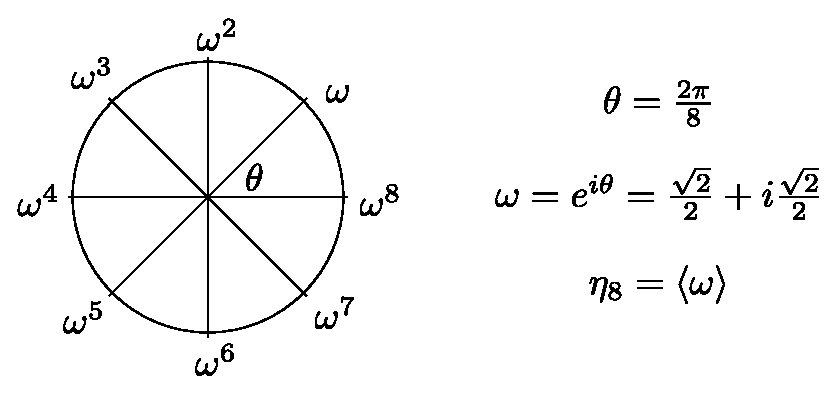
\includegraphics[scale=0.6]{fig01.eps}
    \begin{itemize}
        \item $\omega,\omega^3,\omega^5,\omega^7$  tienen orden 8,
        \item $\omega^2,\omega^6$ tienen orden 4,
        \item $\omega^4$ tiene orden 2 y
        \item $\omega^8=1$ tiene orden 1
    \end{itemize}


    \end{multicols}

    Y si factorizamos $t^8-1$ en $\Q[t]$:
    $t^8-1=(t^4-1)(t^4+1)=(t^2-1)(t^2+1)(t^4+1)=(t-1)(t+1)(t^2+1)(t^4+1)$.

    El polinomio $f=t^4+1$ es irreducible en $\Q[t] \Leftrightarrow
    h=f(t+1)=t^4+4t^3+6t^2+4t+2$  es irreducible en $\Q[t]$. Y como $h$ es
    irreducible por el criterio de Einsenstein con $p=2$, $f$ también es
    irreducible.
\end{ej}

\section{Cuerpos de descomposición}

\begin{defin}
    Sean $\K$ un cuerpo y $f\in\K[t]$ un polinomio de grado $n\geq1$. Decimos
    que $\L\supset\K$ es un \textit{cuerpo de descomposición de $f$ sobre $\K$}
    si:
    \begin{itemize}
        \item $f=c(t-\alpha_1)*\ldots*(t-\alpha_n)$ con $\alpha_1,\alpha_n\in\L, c\in \K$
            y
        \item $\L=\K(\alpha_1,\ldots,\alpha_n)$.
    \end{itemize}
\end{defin}

\begin{obs}
    Hemos visto que si $f\in\K$ con $\deg{f}=n$ existe una extensión
    $\K\subseteq\F$ de forma que $f$ se escinde sobre $\F$. Es decir, existen
    $\alpha_1,\ldots,\alpha_n\in \F$ tales que
    $f=c(t-\alpha_1)*\ldots*(t-\alpha_n)$. Tomamos
    $\L=\K(\alpha_1,\ldots,\alpha_n)\subseteq\F$.
\end{obs}

\begin{ej}\hspace{0pt}
    \begin{itemize}
        \item Sea $f=t^2+1\in\Q[t]$,
            \begin{itemize}
                \item $\Q(i)$ es un cuerpo de descomposición de $f$ sobre $\Q$.
                \item Sean $\L=\frac{\Q[x]}{\left<x^2+1\right>}$ y $\alpha=x+\left<
                    x^2+1\right>$ tenemos $f=(t-\alpha)(t+\alpha)$ en $\L[t]$, por lo
                    que $\L=\Q(\alpha)$ y $\L$ es cuerpo de descomposición de $f$ sobre
                    $\Q$.
            \end{itemize}
            Se tiene un isomorfismo $\L\to\Q(i)$ tal que deja fijo a $\Q$ y
            $\alpha\mapsto i$.
        \item Sea $f=(t^2-2)(t^2-3)$, $\L=\Q(\sqrt{2},\sqrt{3})$ es cuerpo de
            descomposición de $f$ sobre $\Q$.
        \item Sean $f=t^3-2$, $\alpha =\sqrt[3]{2}$ y $\omega$ una raíz cúbica
            de $1$. Se tiene que $(\alpha*\omega)^3=\alpha^3\omega^3=\alpha^3=2$
            y \[f=(t-\alpha)(t-\omega\alpha)(t-\omega^2\alpha).\] Entonces
            $\L=\Q(\alpha,\omega\alpha,\omega^2\alpha)=\Q(\alpha,\omega)$ es
            cuerpo de descomposición de $f$ sobre $\Q$.
        \item Sea $f=t^4-2=(t-\sqrt[4]{2})(t+\sqrt[4]{2})(t-i\sqrt[4]{2})
            (t+i\sqrt[4]{2})$. Entonces
            $\L=\Q(\sqrt[4]{2},-\sqrt[4]{2},i\sqrt[4]{2},-i\sqrt[4]{2})=\Q(i,\sqrt[4]{2})$
            es el cuerpo de descomposición de $f$ sobre $\Q$.
        \item El cuerpo de descomposición de $f=t^2+1$
            \begin{itemize}
                \item sobre $\R$ es $\R(i)=\C$ ,
                \item sobre $\Q(\sqrt{2})$ es $\Q(\sqrt{2})(i)=\Q(\sqrt{2},i)$ y
                \item sobre $\C$ es $\C$.
            \end{itemize}
    \end{itemize}
\end{ej}

\begin{tma}
    Sean $\K$ un cuerpo, $f\in \K[t]$ de grado $n\geq1$ y $\L$ un cuerpo de
    descomposición de $f$ sobre $\K$.\\ Entonces $[\L:\K]\leq n!$
\end{tma}

\begin{proof}
    Por inducción sobre $n=\deg{f}$:
    \begin{itemize}[itemindent=32pt]
        \item[Si $n=1$:] $f=at+b=a(t+\frac{b}{a})$ con $a\neq0$ y
            $\L=\K(-\frac{b}{a})=\K \implies [\L:\K]=1$.
        \item[Si $n>1$:] Sea $\L$ un cuerpo de descomposición de $f$ sobre $\K$.
            $\L=\K(\alpha_1,\ldots,\alpha_n)$ con $\alpha_1,\ldots,\alpha_n$ las
            raíces de $f$. Sea $\F=\K(\alpha_1)$, $\K\subseteq\F\subseteq\L$.

            Tenemos $f=(t-\alpha_1)*g$ en $\F[t]$ ya que $f(\alpha_1)=0$ y
            $\alpha_1\in \F$. Entonces $g\in\F[t]$ y $\deg{g}=n-1$ y
            $\F=(\alpha_2,\ldots,\alpha_n)=\K(\alpha_1)(\alpha_2,\ldots,\alpha_n)
            =\K(\alpha_1,\alpha_2,\ldots,\alpha_n)=\L$ es un cuerpo de
            descomposición de $g$ en $\F$. Aplicando la hipótesis de inducción
            obtenemos que $[\L:\F]\leq (n-1)!$

            Además $[\F:\K]=[\K(\alpha_1):\K]=\deg{m_{\alpha_1,\K}}$ y como
            $f\in \K[t]$ y $f(\alpha_1)=0 \implies m_{\alpha_1,\K}$ divide a $f
            \implies \deg{f}=n\geq\deg{m_{\alpha_1,\K}}=\left[ \F:\K \right]$.

            Con esto se tiene que $[\L:\K]=[\L:\F]*[\F:\K]\leq (n-1)!*n=n!$.
    \end{itemize}
    \vspace{-1em}
\end{proof}

\fecha{8/03} %Copiado de grabación
\begin{defin}[Isomorfismo de extensiones]
    Sean $\varphi: \K_1\to \K_2$ un isomorfismo de cuerpos y
    $\K_1\subseteq\L_1$, $\K_2\subseteq\L_2$ dos extensiones. Decimos que estas
    extensiones son \textit{isomorfas} si existe un isomorfismo
    $\overline{\varphi}:\L_1\to \L_2$ tal que para todo $a\in\K_1$
    \[\overline{\varphi}(a)=\varphi(a).\]
    Es decir, $\K_1\subseteq\L_1$ y $\K_2\subseteq\L_2$ son extensiones
    isomorfas si existe $\overline{\varphi}$ tal que el siguiente diagrama es
    conmutativo:
    \[\begin{tikzcd}
        \L_1\arrow{r}{\overline{\varphi}}  & \L_2 \\%
        \K_1 \arrow{r}{\varphi}\arrow[hook]{u}& \K_2\arrow[hook]{u}
    \end{tikzcd}\]
\end{defin}

\begin{obs}
    Si $\varphi:\K_1 \to \K_2$ es un isomorfismo, sea $f=\sum_{j=0}^ma_jt^j\in
    \K_1[t]$ definimos $\tilde{\varphi}(f)\coloneqq\sum_{j=0}^m\varphi(a_j)t^j$.

    Se tiene que $\tilde{\varphi}:\K_1[t]\to \K_2[t]$ es un isomorfismo de
    anillos (ejercicio).
\end{obs}

\begin{tma}
    Sean $\K_1$ un cuerpo y $f_1\in\K_1[t]$ de grado $n$, $\L_1$ un cuerpo de
    descomposición de $f_1$ sobre $\K_1$, $\varphi:\K_1\to\K_2$ un isomorfismo,
    $f_2=\tilde{\varphi}(f_1)\in\K_2[t]$ y $\L_2$ un cuerpo de descomposición de
    $f_2$ sobre $\K_2$. Entonces las extensiones $\K_1\subseteq\L_1$ y
    $\K_2\subseteq\L_2$ son isomorfas.
\end{tma}

\begin{proof}
    Por inducción sobre $n=\deg{f_1}=\deg{f_2}$.
    \begin{itemize}[itemindent=30pt]
        \item[Si $n=1$.] Entonces $\L_1=\K_1$, $\L_2=\K_2$ y $\varphi:\L_1\to
            \L_2$ es un isomorfismo.
        \item[Si $n>1$.] Sea $f_1=c_1(t-\alpha_1)*\ldots*(t-\alpha_n)$ en
            $\L_1$. La idea es considerar las extensiones intermedias
            $\K_1\subseteq\K_1(\alpha_1)\subseteq\K_1(\alpha_1,\ldots,\alpha_n)=\L_1$
            y construir isomorfismos de extensiones intermedios.
            \begin{enumerate}[itemindent=24pt]
                \item[Paso I.] Modelo abstracto para $\K_1(\alpha_1)$.

                    Sea $h_1=m_{\alpha_1,\K_1}\in\K_1[t]$ tenemos que
                    $h_1\mid f_1$ en $\K_1[t]$ ya que $f_1(\alpha_1)=0$.
                    Como $\alpha_1$ es algebraico tenemos además que
                    $\K_1(\alpha_1)=\K_1[\alpha_1]\cong
                    \frac{\K_1[t]}{\left<h_1\right>}$ mediante el isomorfismo
                    \begin{align*}
                        \psi_1: \K_1[\alpha_1]&\to \frac{\K_1[t]}{\left< h_1
                        \right>}\\
                            \alpha_1&\mapsto t\mod\left<h_1\right>.
                    \end{align*}
                \item[Paso II.] \textit{Tomamos} una raíz de $f_2$
                    correspondiente a $\alpha_1$.

                    Hemos visto que el isomorfismo $\varphi:\K_1\to \K_2$ induce
                    otro isomorfismo $\tilde{\varphi}:\K_1[t]\to\K_2[t]$. Por
                    definición $f_2=\tilde{\varphi}(f_1)$. Como $h_1\mid
                    f_1\implies
                    h_2\coloneqq\tilde{\varphi}(h_1)\mid\varphi(f_1)=f_2$. En
                    $\L_1[t]$ podemos factorizar
                    $f_2=c_2(t-\beta_1)*\ldots*(t-\beta_m)$ y como $h_2\mid
                    f_2$, las raíces de $h_2$ son raíces de $f_2$.
                \item[Paso III.] Modelo para $\K_2(\beta_1)$.

                    Como $h_2\in\K_2[t]$  y $h_2=m_{\beta_1,\K_2}$ tenemos que
                    $\K_2(\beta_1)=\K_2[\beta_1]$ es isomorfo a
                    $\frac{\K_2[t]}{\left< h_2 \right> }$ mediante el
                    isomorfismo
                    \begin{align*}
                        \psi_2: \K_2[\beta_1]&\to \frac{\K_2[t]}{\left< h_2
                        \right>}\\
                            \beta_2&\mapsto t\mod\left<h_2\right>.
                    \end{align*}

                \item[Paso IV.] Las extensiones $\K_1\subseteq\K_1(\alpha_1)$ y
                    $\K_2\subseteq\K_2(\beta_1)$ son isomorfas.

                    Como $h_2=\tilde{\varphi}(h_1)$ y
                    $\tilde{\varphi}:\K_1[t]\to \K_2[t]\implies\left<h_2\right>
                    = \left< \tilde{\varphi}(h_2) \right> $ y obtenemos un
                    isomorfismo \[\hat{\varphi}:\frac{\K_1[t]}{\left<h_1\right>}
                    \to \frac{\K_2[t]}{\left<h_2\right>}\] tal que
                    $\hat{\varphi}(t+\left< h_1 \right> )=t+\left< h_2 \right>$
                    y $\hat{\varphi}(a)=\varphi(a)$ para toda $a\in\K_1$.

                    Juntando lo visto hasta ahora tenemos un isomorfismo
                    $\varphi_1$:
                    \[\begin{tikzcd}
                        \K_1\ar{r}{\psi_1}\ar[bend right]{rrr}{\varphi_1}&
                    \frac{\K_1[t]}{\left<h_1\right>}\ar{r}{\hat{\varphi}}&
                    \frac{\K_2[t]}{\left<h_2\right>}\ar{r} {\psi_2^{-1}}&
                        \K_2(\beta_1)
                    \end{tikzcd}\]
                    tal que $\varphi_1(\alpha_1)=\beta_1$ y
                    $\varphi_1(a)=\varphi(a)$ para toda $a\in\K_1$.

                    Por otro lado, podemos factorizar:
                    \begin{align*}
                        f_1=(t-\alpha_1)*g_1\text{ en }\K_1(\alpha_1)[t]\\
                        f_2=(t-\beta_1)*g_2\text{ en }\K_2(\beta_1)[t]
                    \end{align*}
                    con $\deg{g_1}=\deg{g_2}=n-1$. Ahora
                    $\L_1=\K_1(\alpha_1,\ldots,\alpha_m)=\K_1(\alpha_1)(\alpha_2,
                    \ldots,\alpha_m)$ es un cuerpo de descomposición de $g_1$
                    sobre $\K_1(\alpha_1)$ y $\L_2=\K_2(\beta_1,\ldots,\beta_m)$
                    es un cuerpo de descomposición de $g_2$ sobre
                    $\K_2(\beta_1)$. Si consideramos \[\tilde{\varphi_1}:
                    \K_1(\alpha_1)[t]\to\K_2(\beta_1)[t],\] por lo visto en los
                    pasos anteriores, tenemos que $\tilde{\varphi_1}(f_1)=f_2$ y
                    $\tilde{\varphi_1}(t-\beta_1)=t-\beta_1 \implies
                    \tilde{\varphi_1}(g_1)=g_2$.
                \item[Paso V.] Aplicamos la hipótesis de inducción a
                    $g_1\in\K_1(\alpha_1)[t]$, su cuerpo de descomposición
                    $\L_1$, $g_2\in\K_2(\beta_1)[t]$, su cuerpo de
                    descomposición $\L_2$ y $\varphi_1:\K_1(\alpha_1)\to
                    \K_2(\beta_1)$.

                    Por tanto existe un isomorfismo $\overline{\varphi}:
                    \L_1\to\L_2$ tal que para todo $b\subseteq\K_1(\alpha_1)$ se
                    tiene $\overline{\varphi}(b)=\varphi_1(b)$ y por tanto
                    $\overline{\varphi}(a)=\varphi_1(a)$ para toda $a\in\K_1$.

                    \completar
            \end{enumerate}
    \end{itemize}
\end{proof}

\fecha{10/03}
\begin{cor}
    Sea $\K$ un cuerpo y $f\in\K[t]$ de grado $n\geq1$. Sean $\L$ y $\L'$
    cuerpos de descomposición de $f$ sobre $\K$. Entonces las extensiones
    $\K\subseteq\L$ y $\K\subseteq\L'$ son isomorfas. Es decir existe un
    isomorfismo $\sigma:\L\to\L'$ tal que $\sigma_{\mid_\K}=\id_\K$.
\end{cor}

\begin{proof}
    Tenemos los isomorfismos $\varphi=\id_\K:\K\to\K$ y
    $\tilde{\varphi}=\id_{\K[t]}, \tilde{\varphi}(f)=f$. Aplicando el teorema
    existe un isomorfismo $\sigma:\L\to\L'$ tal que $\sigma(a)=a$ para toda
    $a\in\K$. Es decir, existe $\sigma$ tal que el siguiente diagrama es
    conmutativo:
    \[\begin{tikzcd}
        \L\arrow{r}{\sigma}  & \L' \\%
        \K \arrow{r}{\id_\K}\arrow[hook]{u}& \K\arrow[hook]{u}
    \end{tikzcd}\]
\end{proof}

\begin{cor}
    Sea $\K$ un cuerpo, $f\in\K[t]$ irreducible y $\alpha,\beta$ raíces de $f$
    en su cuerpo de descomposición $\L$ sobre $\K$. Entonces se tiene un
    isomorfismo de cuerpos $\sigma:\L\to\L$  tal que
    $\sigma(\alpha)=\sigma(\beta)$ y $\sigma(a)=a$ para toda $a\in\K$.
\end{cor}

\begin{proof}
    Como $f\in\K[t]$ es irreducible y $\alpha,\beta\in\L$ son raíces de $f$ en
    $\L$ tenemos que $f=m_{\alpha,\K}=m_{\beta,\K}$. Tenemos los isomorfismos
    $\varphi_1$ y $\varphi_2$:
    \[\begin{tikzcd}
        \K(\alpha)=\K[\alpha]\arrow{d}{\varphi_2^{-1}\circ\varphi_1}
        \arrow{r}{\varphi_1}&\frac{\K[t]}{\left<f\right>},\
        \text{ con }\varphi_1(\alpha)=t+\left<f\right>
        \text{ y }\varphi_1(a)=a\ \forall a\in\K;
        \\
        \K(\alpha)=\K[\beta] \arrow{r}{\varphi_1}&\frac{\K[t]}{\left<f\right>},\
        \text{ con }\varphi_2(\beta)=t+\left<f\right>
        \text{ y }\varphi_2(a)=a\ \forall a\in\K.
    \end{tikzcd}\]

    Y el isomorfismo $\varphi\coloneqq\varphi_2^{-1}\circ\varphi_1:\K(\alpha)\to
    \K(\beta)$ es tal que $\varphi(\alpha)=\beta$ y $\varphi(a)=a$ para toda
    $a\in\K$. Observamos además que $\tilde{\varphi}(f)=f$ ya que $f\in\K[t]$ y
    $\varphi_{1\mid_\K}$, $\varphi_{2\mid_\K}$

    \completar

\end{proof}

\begin{ej}
    \begin{itemize}
        \item Sea $f=t^2-2\in\Q[t]$ irreducible y con raíces $\pm\sqrt{2}$.
            $\L=\Q(\sqrt{2})$ es un cuerpo de descomposición de $f$ sobre $\Q$.
            El corolario garantiza que existe un isomorfismo de anillos $\sigma:
            \L\to\L$ tal que $\sigma(\sqrt{2})=-\sqrt{2}$ y $\sigma(a)=a$ para
            toda $a\in\Q$. \[\sigma(a+b\sqrt{2})=\sigma(a)+\sigma(b)
            \sigma(\sqrt{2})=a-b\sqrt{2}\]
        \item Sabemos que $f=t^4-10t^2+1\in\Q[t]$ es irreducible con raíces
            $\pm\sqrt{2},\pm\sqrt{3}$ y cuerpo de descomposición
            $\L=\Q(\sqrt{2}, \sqrt{3})=\Q(\sqrt{2}+\sqrt{3})$.
    \end{itemize}
\end{ej}

\begin{ejer}
    Probar que existe un isomorfismo $\sigma:\L\to\L$ tal que
    $\sigma(\sqrt{2})=\sqrt{2}$ y $\sigma(\sqrt{3})=-\sqrt{3}$.
\end{ejer}

\begin{obs}
    Si $f=a_0+a_1t+\ldots+a_nt^n\in\K[t]$ de grado $n\geq1$ y $\L$ es
    \textit{el} cuerpo de descomposición de $f$ sobre $\K$. Sea $\sigma:\L\to\L$
    un isomorfismo tal que $\sigma(a)=a$ para toda $a\in\K$. Entonces $\sigma$
    define una biyección del conjunto de raíces de $f$ en sí mismo.
\end{obs}
\begin{proof}
    Basta comprobar que si $\alpha$ es raíz de $f$ entonces $\sigma(\alpha)$ es
    raíz de $f$ (ejercicio).
\end{proof}

\fecha{11/03}

Recordemos que, sean $\K$ un cuerpo, $f\in\K[t]$ y $a\in\K$ una raíz de $f$,
existe $m\geq1$ (\textit{la multiplicidad algebraica}) tal que $f=(t-a)^m*h$ con
$h\in\K[t]$ y $h(a)\neq0$. Si $m=1$ decimos que la raíz $a$ es \textit{simple},
y si $m>1$ es \textit{múltiple}.

\begin{defin}[Derivada formal]
    Sea $f=a_nt^n+\ldots+a_1t+a_0\in\K[t]$ su \textit{derivada formal} es el
   polinomio $f'=na_nt^{n-1}+\ldots+a_1\in\K[t]$.
\end{defin}

\begin{prop}
    Sea $\K$ un cuerpo y $f\in\K[t]$ con $\deg{f}\geq1$. Son equivalentes
    \begin{enumerate}
        \item $f$ tiene una raíz múltiple en su cuerpo de descomposición $\L$.
        \item $\mcd{f,f'}\neq 1$. Es decir $f$ y $f'$ tienen un factor
            irreducible en común.
    \end{enumerate}
\end{prop}

\begin{proof}
    Si escribimos $f=(t-a)^m*h$ en $\L[t]$, donde $a\in\L$ y $m$ es la
    multiplicidad algebraica de $a$,
    \[f'=m(t-a)^{m-1}+(t-a)^m*h'=(t-a)^{m-1}(m*h+(t-a)*h').\]
    Si $m=1$, $f'(a)=h(a)\neq 0$ y $m_{\alpha,\K}$ divide a $f$ porque $f(a)=0$,
    pero $m_{\alpha,\K}$ no divide a $f'$ ya que $f'(a)\neq 0$. Como los
    factores irreducibles de $f$ son de la forma $m_{\alpha,\K}$ para $a\in\L$
    raíz de $f$, concluimos que $\mcd{f,f'}=1\Leftrightarrow$ el polinomio $f$
    tiene raíces simples en $\L$.
\end{proof}

\section{Paréntesis: cuerpos finitos}

Sea $\K$ un cuerpo. Tenemos un homomorfismo de anillos $\psi:\Z\to\K$ dado por
\[\psi(n)=n*1_\K=
    \begin{cases}
        1+\stackrel{(n)}{\ldots}+1& \text{ si } n>0\\
        0& \text{ si } n=0\\
        (-1)+\stackrel{(n)}{\ldots}+(-1)& \text{ si } n<0
    \end{cases}
\]

Se dan los siguientes dos casos:
\begin{enumerate}
    \item $\ker{\psi}=\left\{ 0 \right\}$ y $\psi$ es inyectiva, con lo que
        $\Z\subseteq\K \implies \Q\subseteq\K$ y $\K$ tiene característica 0.
    \item $\ker{\psi}=p\Z$ es un ideal de $\Z$ donde $p\neq 0$ es primo. En este
        caso \[\frac{\Z}{\ker{\psi}}=\frac{\Z}{p\Z}\cong\text{un subanillo de
        }\K\] y $p$ es la característica de $\K$. Denotamos por $\F_p=\frac{\Z}
        {p\Z}$ al cuerpo finito con $p$ elementos. Con esto se tiene la
        extensión de cuerpos $\F_p\subseteq\K$.
\end{enumerate}

\begin{ej}
    Sea $\K$ el cuerpo de fracciones del anillo de polinomios $\F_p[x]$ se tiene
    la extensión $\F[x]\subseteq\K$ y como $\F_p\subseteq\K$, $\K$ es un cuerpo
    infinito de característica $p$.
\end{ej}

\begin{obs}
    Si $\car{\K} = p>0$ y  $\varphi:\K\to\K$ es un isomorfismo,
    $\varphi_{\mid_{\F_p}}=\id_{\F_p}$ ya que $\varphi(1)=1$ por definición.
\end{obs}

\begin{obs}
    Sea $\K$ un cuerpo de característica $p>0$. Para todos $a,b\in\K$ y toda
    $n\geq1$ se tiene
    \begin{itemize}
        \item $(a+b)^p=a^p+b^p$ y
        \item $(a+b)^{p^n}=a^{p^n}+b^{p^n}$.
    \end{itemize}
\end{obs}

\begin{proof}
    Usando el binomio de Newton,
    \[(a+b)^p=a^p+\binom{p}{1}a^{p-1}b+\ldots+\binom{p}{p-1}ab^p+b^p\] y
    $\binom{p}{k}=\frac{p!}{k!(p-k)!}=p \frac{(p-1)!}{k!(p-k)!}=0$ en $\K$ ya
    que $\frac{(p-1)!}{k!(p-k)!}\in\N$ y $\car{\K}=p$.
\end{proof}

\begin{defin}
    Sea $\K$ un cuerpo de característica $p$. La aplicación $F:\K\to\K$ tal
    que $F(a)=a^p$ es un homomorfismo que se denomina \textit{homomorfismo de
    Frobenius}.
\end{defin}

\begin{obs}
    El homomorfismo de Frobenius es realmente un homomorfismo ya que
    \begin{itemize}
        \item $F(ab)=(ab)^p=a^pb$
        \item $F(a+b)=(a+b)^p=a^p+b^p$
        \item $F(1)=1^p=1$
    \end{itemize}
\end{obs}

\fecha{15/03}
\begin{obs}
    Sabemos que si $\car{\K}=p$ entonces $\F_p=\left\{
    \overline{1},\ldots,\overline{p-1},\overline{p}=0\right\}\subseteq\K$. Si
    $a\in\F_p$ entonces $F(a)=a^p=a$, y si $a\neq0$ $a^{p-1}=1\mod p$ por el
    \textit{Pequeño teorema de Fermat} $\implies a^p=a$, es decir $F_{|_{\F_p}}=
    \id_{\F_p}$.

    Visto de otra forma, $F(\F_p)\subseteq\F_p$ ya que $F(1)=1$, $F(0)=0$ y al
    ser $F$ un homomorfismo inyectivo de $\F_p\to\F_p$ y $\#\F_p=p$, $F$ tiene
    que ser sobreyectivo.
\end{obs}

\begin{tma}
    Sea $p$ primo y $q=p^n$ con $n\geq1$.
    \begin{enumerate}
        \item El cuerpo de descomposición de $f=t^{p^n}-t$ tiene $q=p^n$
            elementos.
        \item  Si $\K$ es un cuerpo finito de característica $p$ entonces
            $\#\K=p^n$ donde $n=\left[ \K:\F_p \right]$.
        \item Dos cuerpos finitos con $p^n$ elementos son isomorfos
    \end{enumerate}
\end{tma}

\begin{proof}\hspace{0pt}
    \begin{enumerate}
        \item[(2)] $\F_p\subseteq\K \implies \left[ \K:\F_p \right]=n\in\N$. Sea
            $\alpha_1,\ldots, \alpha_n$ una base de $\K$ sobre $\F_p$, si
            $\alpha\in\K$, $\alpha=a_1\alpha_1+\ldots+a_n\alpha_n$ de forma
            única con $a_j\in\F_p$. Es decir, $(a_1,\ldots,a_n)\in\F_p^n$ son
            las coordenadas de $\alpha \implies$ $\#\K=\#\F_p^n=p^n$.
        \item[(1)] $f'=p^nt^{p^n-1}-1$ y como $\car{\K}=p$ $f'=-1$. De aquí
            obtenemos que $\mcd{f,f'}=1$ y por tanto $f$ tiene sólo raíces
            simples en su cuerpo de descomposición $\L$. Sea ahora $M$ el
            conjunto de las raíces de $f$ en $\L$ veamos que $M$ es un cuerpo:
            \begin{itemize}
                \item $1$ es raíz de $f$
                \item Si $\alpha,\beta\in M\implies \alpha,\beta\in M$ ya que
                    $(\alpha\beta)^{p^n}=\alpha^{p^n}\beta^{p^n}=\alpha\beta
                    \implies\alpha\beta\in M$.
                \item Si $\alpha,\beta\in M\implies \alpha+\beta\in M$ ya que
                    $(\alpha+\beta)^{p^n}=\alpha^{p^n}+\beta^{p^n}=\alpha+\beta
                    \implies\alpha+\beta\in M$.
                \item Con los puntos anteriores tenemos que $M$ es un subanillo
                    íntegro con un número finito de elementos. Queda como
                    ejercicio ver que esto implica que $M$ es un cuerpo.
            \end{itemize}
        \item[(3)] Si $\K$ es un cuerpo finito con $\car{\K}=p$ y $p^n$
            elementos, entonces $\K$ es un cuerpo de descomposición de $f$ sobre
            $\F_p$. Sea $\K^\star=\left( \K\setminus\left\{ 0 \right\} , *
                \right)$ grupo con $p^n-1$ elementos, por el \textit{teorema de
            Lagrange}, si $a\in\K\implies s=\ord{a}=\left|\left<a\right>
            \right|\mid \left| \K^\star \right| =p ^n \implies p^n-1=s*t,
            a^{p^n-1}=a^{st}=(a^s)^t=1^t=1\implies a$ es raíz de
            $f=t(t^{p^n-1}-1)$. Si $a=0$, $0$ es raiz de $f$. Todos los
            elementos de $\K$ son raíces de $f$ y como hay exactamente
            $p^n=\#\K$ raíces, $\K$ es cuerpo de descomposición de $f$ sobre
            $\K$. Con esto tenemos el resultado, por la unicidad del cuerpo de
            descomposición.
    \end{enumerate}
\end{proof}

\fecha{16/03} % Ver grabación: problema 15

\begin{notacion}
    Hemos visto que si $p\in\N$  es primo y $n\geq1$ existe un cuerpo $\K$ con
    $q=p^n$ elementos único salvo isomorfismo. Lo denotamos por $\F_q$.
\end{notacion}

\begin{defin}[Función de Euler]
    La \textit{función de Euler} $\phi:\N^+\to\N$ está definida por $\phi(1)=1$
    y para todo $n>1$ $\phi(n)=\#\left\{1\leq j<n\mid \mcd{j,n}=1\right\}=
    \left| \left( \Z_n^\star \right)\right|$.
\end{defin}

\begin{lema}
    Sea $G=\left< a \right> $  un grupo cíclico de orden $m\in\N$.
    \begin{enumerate}
        \item  Para cada divisor $d$ de $m$ existe un único subgrupo de orden
            $d$ de $G$ que además es cíclico.
        \item El número de elementos de orden $m$ en $G$ es $\phi(m)$.
        \item $m=\sum_{d\mid m}\phi(d)$.
    \end{enumerate}
\end{lema}

\begin{proof}\hspace{0pt}
    \begin{enumerate}
        \item[(2)] Usamos la fórmula
            $\ord{a^k}=\frac{\ord{a^k}}{\mcd{k,\ord{a}}}=
            \frac{m}{\mcd{k,m}}$: $\ord{a^k}=m\Leftrightarrow\mcd{k,m}=1$.
            \item[(1)] Supongamos $m=ds$. Se tiene $\ord{a^s}=d$ por la fórmula
                y además $\left< a^s \right> $ tiene orden $d$.
                Sea $H<G$ con $\left|H\right|=d$ y $k=\min\left\{ j\geq1\mid
                a^j\in H \right\}$. Si $a^j\in H$, $j=qk+r$ con $q\in\N$ y
                $0\leq r<k$. Ahora $a^j=(a^k)^q*a^r\implies a^r=a^{j-qk}\in
                H\implies r=0$ (si $r\neq0$ se contradice la definición de
                $k$).

                Por tanto $H= \left< a^k \right>$,
                $\ord{a^k}=\frac{ds}{\mcd{k,m}=d}$ y como $s=\mcd{k,m}\implies
                s\mid k\implies \left<a^k\right>\subseteq \left< a^s\right>$.
                Como ambos tienen orden $d$, $\left<a^k\right>=\left<a^s\right> =H$
            \item[(3)] Si $d=m$, $\phi(m)$ es el número de elementos de orden
                $m$ en $G=\left<a\right>$.

                Si $d<m$, $\phi(d)$ es el número de elementos de orden $d$ en
                $G$, por el apartado (1).
    \end{enumerate}
\end{proof}

\begin{tma}
    El grupo de unidades de $\F_q$ $\left( \F_q^\star=\F_q\setminus\left\{ 0
    \right\},*\right)$ es cíclico.
\end{tma}

\begin{proof}
    Sea $\K$ un cuerpo con $\#\K=p^n=q$ tenemos $\left|\K^\star\right|=q-1$. Sea
    $a\in\K^\star$ con $\ord{a}=d \implies a^d=1 \implies a$ es raíz de
    $t^d-1\in\K[t]$. Sea $1\leq s\leq d$, $a^s\in\left<a\right>$ y $(a^s)^d=1$,
    por lo que $a^s$ también es raíz de $t^d-1$. Por tanto se tiene la siguiente
    descomposición: \[t^d-1=\prod_{j=1}^{d}(t-a^j).\]
    Ahora, si $b\in\K^\star$ y $\ord{b}=d$, entonces $\left<a\right> = \left<b
    \right>$. Si $d$ divide a $\left| \K^\star \right| = q-1$ entonces, sea
    \[c_d=\text{número de elementos de orden }d\text{ en }\K^\star=
        \begin{cases}
            \phi(d)&\text{si }\exists a\in\K \text{ con }\ord{a}=d,\\
            0&\text{en caso contrario}.
        \end{cases}\]
        Como $\left|\K^\star\right|=q-1=\sum_{d\mid q-1} c_d\leq \sum_{d\mid
        q-1}\phi(d)=q-1$ (por el lema anterior) se tiene que $c_d=\phi(d)$ para
        toda $d$ que divida a $q-1$. Por tanto, si $d=q-1,\ c_d=\phi(q-1)\neq0
        \implies\exists\alpha\in\K^\star$ con $\ord{\alpha}=q-1\implies
        \left<\alpha\right>=\K^\star$.
\end{proof}

\fecha{17/03}
\begin{ej}
    Sea $\L=\F_2[t]/\left<f\right>$ con $f=t^4+t^3+t^2+t+1$ y $\alpha=t+\left<f
    \right>$. Entonces $1,\alpha,\alpha^2,\alpha^3$ son base de $\L$ sobre
    $\F_2$ y $\L=\left\{a_0+a_1\alpha+a_2\alpha^2+a_3\alpha^3|a_i\in\F_2
    \right\}$. Tenemos entonces que $\L=\F_{2^4}$ y $\left|\L^\star\right|=15$.

    Buscamos un elemento en $\L^\star$ de orden $15$. Calculamos las potencias
    de $\alpha$ y vimos que $\ord{\alpha}=5$. Sea $\beta=\alpha+1$, $\ord{\beta}
    \mid 15\implies\ord{\beta}\in\left\{1,3,5,15\right\}$. Ahora
    \begin{align*}
        \beta^2&=(\alpha+1)^2=\alpha^2+1,\\
        \beta^3&=(\alpha^2+1)(\alpha+1)=\alpha^3+\alpha^2+\alpha+1,\\
        \beta^5&=\beta^2*\beta^3=(\alpha^2+1)(\alpha^3+\alpha^2+\alpha+1)=
        \alpha^5+\alpha^4+\alpha^3+\alpha^2+\alpha^3+\alpha^2+\alpha+1\\
               &=1+\alpha^3+\alpha^2+\alpha+1+\alpha+1=1+\alpha^3+\alpha^2\neq1
    .\end{align*}
    Donde hemos usado que $f(\alpha)=0\implies
    \alpha^4=\alpha^3+\alpha^2+\alpha+1$. Por tanto concluimos que
    $\ord{\beta}=15$.

    Habíamos visto que $g=t^4+t^3+1=m_{\beta,\F_2}$. Ahora
    \begin{align*}
        \K=\frac{\F_2[t]}{\left<g\right>}&\cong\F_2[\beta]=\L\\
        t+\left<g\right>&\to\beta
    \end{align*}
    y $ord{t+\left< g \right>}=15$ en $\K^\star$. Por tanto $\K^\star=\L^\star$.
\end{ej}

\begin{defin}
    Sea $\F_q$ con $q=p^n$ un cuerpo finito, decimos que $\alpha\in\F$ es
    \textit{primitivo} si \[\left<\alpha\right>=\F_q^\star\Leftrightarrow \F_q
    =\left\{0\right\}\cup\left\{\alpha,\alpha^2,\ldots,\alpha^{n-1}=1\right\}.\]
\end{defin}

\begin{obs}
    El teorema anterior garantiza que para todo cuerpo finito existe
    $\alpha\in\F_q$ primitivo. Si $\alpha\in\F_q$ es primitivo en $\F_q$
    entonces $\alpha^k$ es primitivo $\Leftrightarrow\mcd{k,q-1}=1$.
\end{obs}

\begin{lema}
    Si $g\in\F_p[t]$ y $\alpha\in\K\supset\F_p$ entonces $g(\alpha)=0\implies
    g(\alpha^p)=0$.
\end{lema}

\begin{proof}
    Si $g=a_0+a_1t+\ldots+a_nt^n$,
    $0=g(\alpha)=a_0+a_1\alpha+\ldots+a_n\alpha^n$. Elevando a $p$ y usando que
    $\car{\K}=p$ y $a^p=a$ para toda $a\in\F_p$:
    \[0=(\sum_{i=0}^n a_i\alpha^i)^p=\sum_{i=0}a_i^p\alpha^{ip}=\sum_{i=0}^n
        a_i(\alpha^p)^i=g(\alpha^p).\]
\end{proof}

\begin{ej}
    Sea $\beta\in\L$ una raíz de $g=t^4+t^3+1=(t-\beta)(t-\beta^2)(t-\beta^4)
    (t-\beta^8)$ en $\L[t]$, con $\car{\L}=2$.
    \begin{align*}
        \beta^2 &\text{ es raíz de } g,\\
        \beta^4=(\beta^2)^2 &\text{ es raíz de } g,\\
        \beta^8 &\text{ es raíz de } g \text{ y}\\
        \beta^16=\beta.
    \end{align*}
    Y por tanto $\ord{\beta}=15$.
\end{ej}

\begin{cor}
    Sea $p \in\N$ un número primo:
    \begin{enumerate}
        \item  Para todo $n\in\N$ existe un polinomio irreducible de grado $n$
            en $\F_p[t]$.
        \item Sea $g\in\F_p[t]$ mónico e irreducible con $\deg{g}=n$. Entonces
            \begin{enumerate}
                \item $g$ divide a $f_n=t^{p^n}-t$ y
                \item  $g$ se descompone completamente en $\F_{p^n}[t]$:
                    \[g=(t-\alpha_1)*\ldots*(t-\alpha_n)\]
                    con $\alpha_i\in\F_{p^n}$.
            \end{enumerate}
    \end{enumerate}
\end{cor}

\begin{proof}\hspace{0pt}
    \begin{enumerate}
        \item  $\L=\F_p[t]/\left<g\right>$  es un cuerpo con $q=p^n$ elementos.
            Sea
            \begin{equation}
                \L\cong\F_q=\left\{ \text{raíces de }f_n\in\F_q[t]\right\}
                \tag{$\star$}
            \end{equation}
            Tenemos que si $\alpha=t+\left< g \right> $ en $\L$ entonces
            $g(\alpha)=0$ y $g=m_{\alpha,\F_p}$. Por $\left( \star \right)$,
            $f(\alpha)=0\implies g\mid f_n$.
        \item \completar %Ver vídeo
    \end{enumerate}
\end{proof}

\fecha{18/03} % Ver grabación: ejercicios 16 y 19
\begin{obs}
    Sea $\alpha\in\F_{p^n}$ primitivo y $g=m_{\alpha,\F_p}$, $n=\deg{g}=\left[
    \F_{p^n}:\F_p\right]$. Por el lema, $g(\alpha)=0)=g(\alpha^p)=0$. Obtenemos
    que las siguientes son raíces de $g$: \[\alpha^{p^0},\alpha^{p^1},(\alpha^p)^p=
    \alpha^{p^2},\ldots,\left(\alpha^{p^{n-2}}\right)^p=\alpha^{p^{n-1}},\]
    y son distintas entre si ya que $\alpha\in\F_{p^{n}}$ es primitivo
    $\Leftrightarrow \ord{\alpha}=p^n-1>p^{n-1}$.

    Más adelante veremos que esta propiedad vale para todo $\alpha\in\F_{p^n}$,
    no necesariemente primitivo.
\end{obs}


\fecha{22/03} % Ver grabación: ejercicio 16 y 20
\begin{obs}
    Sea $p$ donde imo, $n\geq1$, $\gamma\in\F_{p^n}$ y $g=m_{\gamma,\F_{p^n}}$
    donde $k=\deg{g}$. Entonces \[\F_{p^k}\cong\frac{\F_p[t]}{\left< g \right>}
        \cong\F_p[\gamma]\subseteq\F_{p^n}.\] 
\end{obs}

\begin{prop}
    Sea $p$ primo y $n_1,n_2\in\N$. Son equivalentes: 
    \begin{enumerate}
        \item $n_1\mid n_2$ 
        \item $\F_{p^{n_1}}\subseteq \F_{p^{n_2}}$ 
    \end{enumerate}
\end{prop}

\begin{proof}\hspace{0pt}
    \begin{itemize}[itemindent=36pt]
        \item[(2)$\implies$(1)] Tenemos $\F_p\subseteq\F_{p^{n_1}}\subseteq
            \F_{p^{n_2}}$ y por la transitividad del grado
            \[n_2=\left[ \F_{p^{n_2}}:\F_p \right]=
            \left[\F_{p^{n_2}}:\F_{p^{n_1}}\right]*
            \left[ \F_{p^{n_1}}:\F_p\right]=
            \left[\F_{p^{n_2}}:\F_{p^{n_1}}\right]*n_1
            \Leftrightarrow n_1\mid n_2.\] 
        \item[(1)$\implies$(2)] Tenemos $n_2=d*n_1$. Sea $\alpha\in\F_{p^{n_2}}$
            primitivo, $\left< \alpha \right>=\F_{p^{n_2}}^\star$ y
            $\ord{\alpha}=p^{n_2}-1$. Ahora, como $n_2=d*n_1$, $p^{n_1}-1$
            divide a $p^{n_2}-1$ ya que
            $x^d-1=(x-1)(x^{d-1}+x^{d-2}+\ldots+x+1)$ y sustituyendo $x$ por
            $p^{n_1}$,
            \[p^{n_1*d}-1=(p^{n_2}-1)*s\]
            para algún $s\in\Z$.

            Si $\beta=\alpha^s$, como $\ord{\alpha}=p^{n_1*d}-1$, $\ord{
            \beta}={\ord{\alpha}}/{\mcd{\ord{\alpha},s}}=p^{n_1}-1$ y 
            $\beta$ es raíz del polinomio $f_{n_1}=t^{p^{n_1}-1}-t$.
            Como las raíces de $f_{n_1}$ son los elementos de $\F_{p^{n_1}}$ y
            $\ord{\beta}=p^{n_1}-1$,
            \[\F_{p^{n_1}}=\{\beta,\beta^2,\ldots,\beta^{p^{n_1}-1}=1
            \}\cup \left\{ 0 \right\}\subseteq\F_{p^{n_2}}.\] 
    \end{itemize}
\end{proof}

\begin{ejer}
    Hallar los subcuerpos de $\F_{16}$ y $\F_{2^{15}}$.  
\end{ejer}

\fecha{23/03} % Ver grabación y completar el inicio
\begin{ej}
    Consideramos $\F_{2^15}$,
    \completar
\end{ej}

\fecha{24/03} % Ver grabación

\begin{defin}
    Sea $\K\subseteq\L$ una extensión y $\alpha\in\L$ algebraico sobre $\K$.
    Decimos que $\alpha$ es \textit{separable} sobre $\K$ si $m_{\alpha,\K}$ no
    tiene raíces múltiples en su cuerpo de descomposición.
\end{defin}

\begin{obs}
    Si $h\in\K[t]$ tiene grado $\geq1$, son equivalentes:
    \begin{enumerate}
        \item $h$ no tiene raíces múltiples en su cuerpo de descomposición.
        \item $\mcd{h,h'}=1$, es decir h y h' no tienen factores irreducibles
            comunes. 
    \end{enumerate}
\end{obs}

\begin{defin}
    Una extensión $\K\subseteq\L$ es \textit{separable} si todo $\alpha$
    algebraico sobre $\K$ es separable sobre $\K$.  
\end{defin}

\begin{prop}
    Sea $\K\subseteq\L$ una extensión,$\alpha\in\L$.
    \begin{enumerate}
        \item Si $\car\K=0$ entonces $\alpha$ es separable.  
        \item si $\L$ es un cuerpo finito $\alpha$ es separable.
    \end{enumerate}
\end{prop}

\begin{proof}\hspace{0pt}
    \begin{enumerate}
        \item Sea $f=m_{\alpha,\K}\in\K[t]$ de grado $n=[\K(\alpha):\K]\geq1$.
            Por un lado $f=t^n+a_1t^{n-1}+\ldots+a_n$ es irreducible y además
            $f'=nt^{n-1}+a(n-1)t^{n-2}+\ldots+a_{n-1}$ donde $n\neq0$ ya que
            $\car\K=0$. Por tanto, como $\deg{f'}=n-1$ y $f$ es irreducible,
            $\mcd{f,f'}=1$.
        \item Sabemos que existen $q=p^n$ con $p$ primo tales que $\K\cong\F_q$,
            $\L\cong\F_{q^n}=\F_{p^{nm}}$ y $n=[\L:\K]$. Entonces, si
            $\alpha\in\L$, $m_{\alpha,\K}$ divide a $t^{p^{nm}}-t=\prod_{\beta
            \in\L}(t-\beta)$ y por tanto $m_{\alpha,\K}$ tiene solo raíces
            simples. \revisar
    \end{enumerate}
\end{proof}

\begin{ej}[Extensión no separable]
    Sea $\K=\F_p(x)$ el cuerpo de fracciones de $\F_p[x]$. Sabemos que $\K$ es
    infinito y $\car{\K}=p$.

    Sea $f=t^p+x\in\F_p[x][t]$. Aplicando el \textit{criterio de irreducibilidad
    de Eisenstein} para el elemento primo $x\in\F_p[x]$ ($x$ es primo ya que
    $\F_p[x]$ es DFU, por lo que todo irreducible es primo) deducimos que $f$ es
    irreducible.
    Por el \textit{lema de Gauss} sabemos que $f$ es irreducible en
    $\F_p(x)[t]=\K[t]$.  

    Sea $\L$ el cuerpo de descomposición de $f$ sobre $\K$. Tomo $\alpha\in\L$
    una raíz de $f$: $f(\alpha)=\alpha^p+x=0\implies x=\alpha^p$.
    En $\L[t]$, $f=t^p+\alpha^p=(t+\alpha)^p$ ya que $\car{\K}=p$.   

    Por tanto $\L=\K(\alpha)$ y $m_{\alpha,\K}$ tiene una raíz de multiplicidad
    $p>1$, por lo que $\alpha$ no es separable sobre $\K$.   
\end{ej}

\begin{tma}[del elemento primitivo]
    Sea $\K\subseteq\L$ una extensión finita y separable. Entonces existe
    $\alpha\in\L$ tal que $\L=\K(\alpha)$. Además, si $\K$ es infinito y
    $\L=\K(\alpha_1,\ldots,\alpha_n)$, podemos tomar $\lambda_i\in\K$ tales que 
    \[\alpha=\lambda_1\alpha_1+\ldots+\lambda_n\alpha_n.\] 
\end{tma}

\begin{proof}
    Si $\K\subseteq\L$ es una extensión finita, existen
    $\alpha_1,\ldots,\alpha_n\in\L$ tales que $\L=\K(\alpha_1,\ldots,\alpha_n)$.

    Supongamos que $\K$ es infinito y probemos el resultado por inducción sobre
    $n$.
    \begin{itemize}
        \item Empezamos con $n=2$: $\L=\K(\beta,\gamma)$. Sean
            $f=m_{\beta,\K}$ y $g=m_{\gamma,\K}$ con $\deg{f}=l$ y
            $\deg{g}=m$. La separabilidad implica que $f$ tiene $l$ raíces
            distintas $\beta=\beta_1,\ldots,\beta_n$ y $g$ tiene $m$ raíces
            distintas $\gamma=\gamma_1,\ldots,\gamma_n$ en el cuerpo de
            descomposición $\mathbb{M}$ de $f*g$.  
    \end{itemize}
    \completar

\fecha{25/03}
    \completar 
\end{proof}

\begin{ej}
    Sea $\Q(\sqrt{2},\sqrt{3})$, $\beta=\beta_1=\sqrt{2}$, $\beta_2=-\sqrt{2}$ y
    $\gamma=\gamma_1=\sqrt{3}$, $\gamma_2=-\sqrt{3}$. Tenemos
    \[\frac{\beta_i-\beta_j}{\gamma_l-\gamma_s}\in\left\{ 0,\pm\frac{\sqrt{2}
    }{\sqrt{3} }/ \right\}.\]

    La demostración del teorema nos dice que si $\lambda\in\Q\setminus\left\{0
    \right\}$, $\Q(\sqrt{2}+\lambda\sqrt{3})=\Q(\sqrt{2},\sqrt{3})$.
\end{ej}

\begin{ejer}
    Hacer lo mismo con $\Q(\sqrt{2},\sqrt[3]{3})$. 
\end{ejer}


\begin{ej}[extensión no separable]
    \completar % ¿es el mismo ejemplo de ayer?
\end{ej}

\begin{ej}[Extensión infinita que no es simple]
    Sea una extensión $\K\subseteq\K(\beta,\gamma)=\L$ tal que para toda $\alpha
    \in\L$ $\K(\alpha)\neq \L$. Por ejemplo tomamos $\K = $ cuerpo de fracciones
    de $\F_p[x,y]$ (con $x$ e $y$ variables). Sea $\alpha$ una raíz de $t^p-x$ y
    $\beta$ una raíz de $t^p-y$. Como $\F_p[x,y]$ es DFU, $x$ e $y$ son
    irreducibles y $t^p-x$ y $t^p-y$ son irreducibles en $\K[t]$.    

    Queda como ejercicio probar que
    \begin{enumerate}
        \item $\left[ \K(\alpha,\beta):\K \right] =p^2$ y
        \item si $\gamma\in\K(\alpha,\beta)$ entonces $\gamma^p \in\K$ y por
            tanto $m_{\gamma,\K}$ divide a $t^p-\gamma^p$, lo que implica que
            $[\K(\gamma):\K]\leq p$.  \end{enumerate}
\end{ej}




\end{document}
